% =====================================================================
%  SIREN: Hearing the Loud Answer Instead of the Right One
%
%  Every quantitative value is a macro from numbers.tex, generated by
%  make_numbers.py from UNDERTONE_report/data/.  The prose states no
%  item count; counts appear only in table columns.  To update after a
%  new run:  python make_numbers.py && tectonic siren.tex
%
%  Benchmark name, corpus list and author block are the three macros
%  directly below.
% =====================================================================
\documentclass{article}
\usepackage{amsmath,amssymb,graphicx,booktabs,multirow,url}
% Venue style: replace the four lines below with \usepackage{spconf} (or the
% venue's class) when submitting; they emulate a two-column 9pt layout.
\makeatletter\@twocolumntrue\makeatother
\usepackage[letterpaper,margin=0.72in]{geometry}
\newcommand{\ninept}{\fontsize{9}{10}\selectfont}
\newcommand{\name}[1]{\author{#1}}
\newcommand{\address}[1]{\date{#1}}
\newenvironment{keywords}{\par\noindent\textbf{Index Terms---}\ignorespaces}{\par}
\usepackage[dvipsnames,table]{xcolor}
\usepackage{tikz}
\usepackage{pgfplots}
\pgfplotsset{compat=1.17}
\usetikzlibrary{arrows.meta,positioning}
\usepackage{pifont}
\usepackage{stfloats}
\newcommand{\cmark}{\ding{51}}
\newcommand{\xmark}{\ding{55}}

\newcommand{\bench}{SIREN}
\newcommand{\corpus}{the AMI Meeting Corpus}
\newcommand{\corpusshort}{AMI}
\newcommand{\plannedcorpus}{ICSI and MeetingBank}

% generated by make_numbers.py - do not edit
\newcommand{\Nitems}{408}
\newcommand{\Nnonnull}{357}
\newcommand{\Nnull}{51}
\newcommand{\Nwindows}{187}
\newcommand{\Nmeetings}{104}
\newcommand{\Nconstructed}{28}
\newcommand{\NcatPOne}{20}
\newcommand{\NcatPTwo}{125}
\newcommand{\NcatPThree}{54}
\newcommand{\NcatPFour}{106}
\newcommand{\NcatCOne}{103}
\newcommand{\Nscenario}{349}
\newcommand{\Nnonscenario}{59}
\newcommand{\NitemsBand}{85}
\newcommand{\Nmodels}{13}
\newcommand{\Nfullcov}{9}
\newcommand{\Ntrunc}{3}
\newcommand{\Nsweeppool}{7}
\newcommand{\Nexcluded}{4}
\newcommand{\Nfamilies}{7}
\newcommand{\Ntwins}{4}
\newcommand{\ladderBody}{\ctr{Qwen2-Audio-7B} & Qwen & 7.0 & \ctr{30\,s} & logit & 0.57 & 0.20 & 0.23 & 0.25 & 0.35 & 0.25 & 0.36 & 0.32 & 0.18 \\
Qwen2.5-Omni-3B & Qwen & 3.0 & $\geq$\,600\,s & logit & 0.59 & 0.51 & 0.36 & 0.40 & 0.23 & 0.23 & 0.31 & 0.35 & 0.27 \\
Qwen2.5-Omni-7B & Qwen & 7.0 & $\geq$\,600\,s & logit & 0.62 & 0.44 & 0.44 & 0.46 & 0.18 & 0.25 & 0.16 & 0.44 & 0.29 \\
Phi-4-multimodal & Microsoft & 5.6 & $\geq$\,600\,s & logit & 0.35 & 0.24 & 0.18 & 0.24 & 0.17 & 0.23 & 0.45 & 0.28 & 0.15 \\
\ctr{Gemma-3n-E2B} & Google & 2.0 & \ctr{30\,s} & logit & 0.58 & 0.18 & 0.17 & 0.23 & 0.41 & 0.18 & 0.53 & 0.21 & 0.06 \\
\ctr{Gemma-3n-E4B} & Google & 4.0 & \ctr{30\,s} & logit & 0.61 & 0.19 & 0.18 & 0.26 & 0.43 & 0.20 & 0.47 & 0.24 & 0.09 \\
\ctr{Aero-1-Audio} & LMMS & 1.5 & \ctr{see \S\ref{ssec:artefacts}} & logit & 0.43 & 0.28 & 0.26 & 0.28 & 0.17 & 0.27 & 0.23 & 0.37 & 0.09 \\
Voxtral-Mini-3B & Mistral & 3.0 & 600\,s & logit & 0.23 & 0.17 & 0.13 & 0.23 & 0.10 & 0.16 & 0.61 & 0.19 & 0.13 \\
MOSS-Audio-4B-Instruct & OpenMOSS & 4.0 & $\geq$\,600\,s & logit & 0.42 & 0.31 & 0.24 & 0.27 & 0.18 & 0.24 & 0.38 & 0.32 & 0.22 \\
MOSS-Audio-4B-Thinking & OpenMOSS & 4.0 & $\geq$\,600\,s & gen & 0.66 & 0.53 & 0.45 & 0.51 & 0.21 & 0.30 & 0.08 & 0.55 & n/a \\
MOSS-Audio-8B-Instruct & OpenMOSS & 8.0 & $\geq$\,600\,s & logit & 0.48 & 0.31 & 0.24 & 0.25 & 0.24 & 0.18 & 0.46 & 0.24 & 0.25 \\
MOSS-Audio-8B-Thinking & OpenMOSS & 8.0 & $\geq$\,600\,s & gen & 0.68 & 0.54 & 0.51 & 0.54 & 0.17 & 0.26 & 0.10 & 0.53 & n/a \\
Audio-Flamingo-Next & NVIDIA & -- & $\geq$\,600\,s & logit & 0.63 & 0.49 & 0.46 & 0.44 & 0.17 & 0.29 & 0.08 & 0.54 & 0.29 \\}
\newcommand{\roleCorrectLOne}{0.52}
\newcommand{\roleSalienceLOne}{0.13}
\newcommand{\roleRecencyLOne}{0.09}
\newcommand{\roleAbsentLOne}{0.26}
\newcommand{\roleCorrectLTwo}{0.39}
\newcommand{\roleSalienceLTwo}{0.22}
\newcommand{\roleRecencyLTwo}{0.12}
\newcommand{\roleAbsentLTwo}{0.27}
\newcommand{\roleCorrectLThree}{0.33}
\newcommand{\roleSalienceLThree}{0.24}
\newcommand{\roleRecencyLThree}{0.14}
\newcommand{\roleAbsentLThree}{0.29}
\newcommand{\roleCorrectLFour}{0.37}
\newcommand{\roleSalienceLFour}{0.26}
\newcommand{\roleRecencyLFour}{0.15}
\newcommand{\roleAbsentLFour}{0.22}
\newcommand{\retrievalCost}{0.18}
\newcommand{\coordsRoles}{(L1,0.516) (L2,0.392) (L3,0.332) (L4,0.370)}
\newcommand{\coordsCorrect}{(L1,0.516) (L2,0.392) (L3,0.332) (L4,0.370)}
\newcommand{\coordsSalience}{(L1,0.129) (L2,0.215) (L3,0.238) (L4,0.260)}
\newcommand{\coordsRecency}{(L1,0.092) (L2,0.125) (L3,0.138) (L4,0.151)}
\newcommand{\coordsAbsent}{(L1,0.262) (L2,0.268) (L3,0.292) (L4,0.220)}
\newcommand{\Sfull}{0.36}
\newcommand{\Siso}{0.27}
\newcommand{\pairCorrectDown}{727}
\newcommand{\pairCorrectUp}{143}
\newcommand{\pairCorrectP}{<10^{-95}}
\newcommand{\pairSalienceDown}{122}
\newcommand{\pairSalienceUp}{464}
\newcommand{\pairSalienceP}{<10^{-48}}
\newcommand{\pairAbsentDown}{287}
\newcommand{\pairAbsentUp}{383}
\newcommand{\pairAbsentP}{=2.4e-04}
\newcommand{\pairRecencyDown}{104}
\newcommand{\pairRecencyUp}{250}
\newcommand{\pairRecencyP}{<10^{-15}}
\newcommand{\pairAbsentOracleDown}{261}
\newcommand{\pairAbsentOracleUp}{39}
\newcommand{\pairAbsentOracleP}{<10^{-41}}
\newcommand{\pairCorrectOracleDown}{92}
\newcommand{\pairCorrectOracleUp}{205}
\newcommand{\pairCorrectOracleP}{<10^{-11}}
\newcommand{\signLThreebelowLOneall}{13/13}
\newcommand{\signLThreebelowLOne}{9/9}
\newcommand{\signDecoyUp}{9/9}
\newcommand{\signDenialUp}{5/9}
\newcommand{\signAudioDep}{7/7}
\newcommand{\signP}{=0.004}
\newcommand{\signPall}{=2.4e-04}
\newcommand{\meanRetrievalCost}{0.18}
\newcommand{\minRetrievalCost}{0.10}
\newcommand{\maxRetrievalCost}{0.24}
\newcommand{\oracleGain}{0.04}
\newcommand{\oracleDenialDrop}{0.07}
\newcommand{\NbandModels}{9}
\newcommand{\lenCorrect}{(20\,s,0.516) (120\,s,0.392) (300\,s,0.332) (600\,s,0.261)}
\newcommand{\lenSalience}{(20\,s,0.129) (120\,s,0.215) (300\,s,0.238) (600\,s,0.268)}
\newcommand{\lenRecency}{(20\,s,0.092) (120\,s,0.125) (300\,s,0.138) (600\,s,0.131)}
\newcommand{\lenAbsent}{(20\,s,0.262) (120\,s,0.268) (300\,s,0.292) (600\,s,0.340)}
\newcommand{\lenBody}{20\,s & within item & 356 & 9 & 0.52 & 0.13 & 0.09 & 0.26 \\
120\,s & within item & 355 & 9 & 0.39 & 0.22 & 0.12 & 0.27 \\
300\,s & within item & 353 & 9 & 0.33 & 0.24 & 0.14 & 0.29 \\
600\,s & separate band & 74 & 9 & 0.26 & 0.27 & 0.13 & 0.34 \\}
\newcommand{\bandCorrIso}{0.52}
\newcommand{\bandCorrFull}{0.26}
\newcommand{\bandDecoy}{0.27}
\newcommand{\bandDenial}{0.34}
\newcommand{\lenSalFirst}{0.13}
\newcommand{\lenSalLast}{0.27}
\newcommand{\lenCorrFirst}{0.52}
\newcommand{\lenCorrLast}{0.26}
\newcommand{\sweepCorrect}{(0,0.415) (-3,0.408) (-6,0.406) (-9,0.401) (-12,0.393) (-18,0.379) (-24,0.343)}
\newcommand{\sweepSalience}{(0,0.187) (-3,0.187) (-6,0.186) (-9,0.188) (-12,0.191) (-18,0.200) (-24,0.208)}
\newcommand{\sweepAbsent}{(0,0.302) (-3,0.306) (-6,0.311) (-9,0.316) (-12,0.324) (-18,0.330) (-24,0.356)}
\newcommand{\sweepRecency}{(0,0.096) (-3,0.099) (-6,0.097) (-9,0.095) (-12,0.092) (-18,0.092) (-24,0.093)}
\newcommand{\sweepCorrz}{0.41}
\newcommand{\sweepSalz}{0.19}
\newcommand{\sweepAbsz}{0.30}
\newcommand{\sweepRecz}{0.10}
\newcommand{\sweepCorrmThree}{0.41}
\newcommand{\sweepSalmThree}{0.19}
\newcommand{\sweepAbsmThree}{0.31}
\newcommand{\sweepRecmThree}{0.10}
\newcommand{\sweepCorrmSix}{0.41}
\newcommand{\sweepSalmSix}{0.19}
\newcommand{\sweepAbsmSix}{0.31}
\newcommand{\sweepRecmSix}{0.10}
\newcommand{\sweepCorrmNine}{0.40}
\newcommand{\sweepSalmNine}{0.19}
\newcommand{\sweepAbsmNine}{0.32}
\newcommand{\sweepRecmNine}{0.09}
\newcommand{\sweepCorrmTwelve}{0.39}
\newcommand{\sweepSalmTwelve}{0.19}
\newcommand{\sweepAbsmTwelve}{0.32}
\newcommand{\sweepRecmTwelve}{0.09}
\newcommand{\sweepCorrmEighteen}{0.38}
\newcommand{\sweepSalmEighteen}{0.20}
\newcommand{\sweepAbsmEighteen}{0.33}
\newcommand{\sweepRecmEighteen}{0.09}
\newcommand{\sweepCorrmTwentyfour}{0.34}
\newcommand{\sweepSalmTwentyfour}{0.21}
\newcommand{\sweepAbsmTwentyfour}{0.36}
\newcommand{\sweepRecmTwentyfour}{0.09}
\newcommand{\sweepCorrmSixty}{0.12}
\newcommand{\sweepSalmSixty}{0.31}
\newcommand{\sweepAbsmSixty}{0.45}
\newcommand{\sweepRecmSixty}{0.12}
\newcommand{\sweepBody}{+0 & 0.41 & 0.19 & 0.10 & 0.30 \\
-3 & 0.41 & 0.19 & 0.10 & 0.31 \\
-6 & 0.41 & 0.19 & 0.10 & 0.31 \\
-9 & 0.40 & 0.19 & 0.09 & 0.32 \\
-12 & 0.39 & 0.19 & 0.09 & 0.32 \\
-18 & 0.38 & 0.20 & 0.09 & 0.33 \\
-24 & 0.34 & 0.21 & 0.09 & 0.36 \\
-60 & 0.12 & 0.31 & 0.12 & 0.45 \\}
\newcommand{\audioDepMean}{0.23}
\newcommand{\audioDepMin}{0.13}
\newcommand{\audioDepMax}{0.29}
\newcommand{\signSweepFall}{7/7}
\newcommand{\signSweepDecoyUp}{7/7}
\newcommand{\signSweepDenialUp}{7/7}
\newcommand{\sweeprmSalience}{0.31}
\newcommand{\sweeprmAbsent}{0.45}
\newcommand{\sweeprmCorrect}{0.12}
\newcommand{\sweeprmRecency}{0.12}
\newcommand{\boostMean}{+0.004}
\newcommand{\boostMin}{+0.000}
\newcommand{\boostMax}{+0.010}
\newcommand{\signBoost}{5/7}
\newcommand{\compMean}{+0.031}
\newcommand{\signComp}{7/7}
\newcommand{\calMean}{-0.016}
\newcommand{\signCal}{6/7}
\newcommand{\boostCurve}{(0,0.415) (3,0.417) (6,0.419) (9,0.420)}
\newcommand{\boostDecoy}{(0,0.187) (3,0.185) (6,0.184) (9,0.183)}
\newcommand{\compCurve}{(0,0.413) (-6,0.414) (-12,0.413) (-24,0.415) (-60,0.446)}
\newcommand{\compDecoy}{(0,0.217) (-6,0.214) (-12,0.214) (-24,0.200) (-60,0.150)}
\newcommand{\calCurve}{(0,0.415) (-2,0.409) (-4,0.410) (-6,0.406) (-8,0.401) (-10,0.400) (-12,0.393)}
\newcommand{\compZero}{0.41}
\newcommand{\compRemoved}{0.45}
\newcommand{\compDecoyZero}{0.22}
\newcommand{\compDecoyRemoved}{0.15}
\newcommand{\boostZero}{0.41}
\newcommand{\boostNine}{0.42}
\newcommand{\twoByTwoBody}{\ctr{Qwen2-Audio-7B} & 0.18 & -0.005 & 0.029 & -0.029 \\
Qwen2.5-Omni-3B & 0.27 & 0.005 & 0.033 & 0.002 \\
Qwen2.5-Omni-7B & 0.29 & 0.007 & 0.023 & -0.007 \\
Phi-4-multimodal & 0.15 & 0.005 & 0.020 & -0.007 \\
\ctr{Gemma-3n-E2B} & 0.06 & 0.010 & 0.010 & -0.002 \\
\ctr{Gemma-3n-E4B} & 0.09 & 0.015 & 0.007 & -0.010 \\
\ctr{Aero-1-Audio} & 0.09 & 0.005 & 0.016 & -0.015 \\
Voxtral-Mini-3B & 0.13 & 0.000 & 0.023 & -0.034 \\
MOSS-Audio-4B-Instruct & 0.22 & 0.000 & 0.026 & -0.039 \\
MOSS-Audio-8B-Instruct & 0.25 & 0.002 & 0.042 & -0.025 \\
Audio-Flamingo-Next & 0.29 & 0.010 & 0.049 & -0.005 \\}
\newcommand{\signAudioDepAll}{11/11}
\newcommand{\NcompItems}{306}
\newcommand{\catPOneCorr}{0.36}
\newcommand{\catPOneDec}{0.16}
\newcommand{\catPOneDen}{0.36}
\newcommand{\catPOneR}{0.33}
\newcommand{\catPTwoCorr}{0.35}
\newcommand{\catPTwoDec}{0.25}
\newcommand{\catPTwoDen}{0.28}
\newcommand{\catPTwoR}{0.22}
\newcommand{\catPThreeCorr}{0.31}
\newcommand{\catPThreeDec}{0.26}
\newcommand{\catPThreeDen}{0.30}
\newcommand{\catPThreeR}{0.21}
\newcommand{\catPFourCorr}{0.27}
\newcommand{\catPFourDec}{0.28}
\newcommand{\catPFourDen}{0.26}
\newcommand{\catPFourR}{0.12}
\newcommand{\catCOneCorr}{0.39}
\newcommand{\catCOneDec}{0.18}
\newcommand{\catCOneDen}{0.31}
\newcommand{\catCOneR}{0.16}
\newcommand{\catBody}{P1 & 18 & 0.70 & 0.36 & 0.33 & 0.16 & 0.12 & 0.36 \\
P2 & 111 & 0.57 & 0.35 & 0.22 & 0.25 & 0.12 & 0.28 \\
P3 & 45 & 0.53 & 0.31 & 0.21 & 0.26 & 0.12 & 0.30 \\
P4 & 95 & 0.39 & 0.27 & 0.12 & 0.28 & 0.19 & 0.26 \\
C1 & 88 & 0.55 & 0.39 & 0.16 & 0.18 & 0.12 & 0.31 \\}
\newcommand{\catRmaxName}{P1}
\newcommand{\catRmaxVal}{0.33}
\newcommand{\catRminName}{P4}
\newcommand{\catRminVal}{0.12}
\newcommand{\catDecMaxName}{P4}
\newcommand{\catDecMaxVal}{0.28}
\newcommand{\catDecMinName}{P1}
\newcommand{\catDecMinVal}{0.16}
\newcommand{\ScenCorrOne}{0.51}
\newcommand{\ScenCorrThree}{0.33}
\newcommand{\ScenDec}{0.22}
\newcommand{\ScenDen}{0.31}
\newcommand{\ScenN}{309}
\newcommand{\NonscenCorrOne}{0.53}
\newcommand{\NonscenCorrThree}{0.37}
\newcommand{\NonscenDec}{0.33}
\newcommand{\NonscenDen}{0.19}
\newcommand{\NonscenN}{48}
\newcommand{\corpusBody}{AMI & 327 & 0.52 & 0.33 & 0.19 & 0.23 & 0.14 & 0.30 \\
ICSI & 30 & 0.51 & 0.36 & 0.15 & 0.34 & 0.14 & 0.16 \\}
\newcommand{\Ncorpora}{2}
\newcommand{\nullSentinelLOne}{0.27}
\newcommand{\nullDecoyLOne}{0.06}
\newcommand{\nullSentinelLThree}{0.28}
\newcommand{\nullDecoyLThree}{0.11}
\newcommand{\nullSentinelLFour}{0.18}
\newcommand{\nullDecoyLFour}{0.13}
\newcommand{\calibGapLThree}{-0.01}
\newcommand{\qogemmaThreeneTwob}{0.16}
\newcommand{\qomossaudioFourbinstruct}{0.05}
\newcommand{\qophiFourmultimodal}{0.02}
\newcommand{\qoqwenTwoFiveomniSevenb}{0.03}
\newcommand{\qogptaudiomini}{0.03}
\newcommand{\qoBody}{Gemma-3n-E2B & 408 & 0.16 & 0.54 & 0.76 \\
MOSS-Audio-4B-Instruct & 408 & 0.05 & 0.88 & 0.98 \\
Phi-4-multimodal & 408 & 0.02 & 0.95 & 0.92 \\
Qwen2.5-Omni-7B & 408 & 0.03 & 0.94 & 1.00 \\
GPT-audio-mini & 407 & 0.03 & 0.91 & 1.00 \\}
\newcommand{\qoPoolAcc}{0.06}
\newcommand{\qoPoolSentinel}{0.83}
\newcommand{\qoNullSentinel}{0.92}
\newcommand{\twinBody}{Whisper$\rightarrow$Qwen2.5-7B & 0.49 & 0.18 & 0.31 & 0.30 & 0.34 \\
Whisper$\rightarrow$Llama-3.1-8B & 0.49 & 0.40 & 0.09 & 0.27 & 0.18 \\
Whisper$\rightarrow$Mistral-7B & 0.43 & 0.25 & 0.18 & 0.32 & 0.30 \\
Whisper$\rightarrow$Gemma-2-9B & 0.57 & 0.38 & 0.19 & 0.32 & 0.11 \\}
\newcommand{\twinCorrOne}{0.49}
\newcommand{\twinCorrThree}{0.30}
\newcommand{\twinDecoyThree}{0.30}
\newcommand{\twinDenialThree}{0.23}
\newcommand{\twinDenialOne}{0.26}
\newcommand{\twinCatBody}{P1 & 0.36 & 0.26 & 0.36 & 0.40 \\
P2 & 0.35 & 0.29 & 0.28 & 0.25 \\
P3 & 0.31 & 0.32 & 0.30 & 0.19 \\
P4 & 0.27 & 0.27 & 0.26 & 0.20 \\
C1 & 0.39 & 0.35 & 0.31 & 0.24 \\}
\newcommand{\twinPairAudioRight}{111}
\newcommand{\twinPairTextRight}{17}
\newcommand{\twinPairP}{<10^{-18}}
\newcommand{\closedgeminiflashCorrOne}{0.76}
\newcommand{\closedgeminiflashCorrThree}{0.66}
\newcommand{\closedgeminiflashDecThree}{0.15}
\newcommand{\closedgeminiflashDenThree}{0.10}
\newcommand{\closedgeminiflashRefusals}{0}
\newcommand{\closedgeminiflashN}{355}
\newcommand{\closedgeminiflashPairDown}{52}
\newcommand{\closedgeminiflashPairUp}{18}
\newcommand{\closedgeminiflashPairP}{<10^{-5}}
\newcommand{\closedgeminiliteCorrOne}{0.64}
\newcommand{\closedgeminiliteCorrThree}{0.48}
\newcommand{\closedgeminiliteDecThree}{0.23}
\newcommand{\closedgeminiliteDenThree}{0.14}
\newcommand{\closedgeminiliteRefusals}{0}
\newcommand{\closedgeminiliteN}{325}
\newcommand{\closedgeminilitePairDown}{71}
\newcommand{\closedgeminilitePairUp}{18}
\newcommand{\closedgeminilitePairP}{<10^{-8}}
\newcommand{\closedgptaudiominiCorrOne}{0.43}
\newcommand{\closedgptaudiominiCorrThree}{0.25}
\newcommand{\closedgptaudiominiDecThree}{0.26}
\newcommand{\closedgptaudiominiDenThree}{0.36}
\newcommand{\closedgptaudiominiRefusals}{51}
\newcommand{\closedgptaudiominiN}{357}
\newcommand{\closedgptaudiominiPairDown}{66}
\newcommand{\closedgptaudiominiPairUp}{14}
\newcommand{\closedgptaudiominiPairP}{<10^{-9}}
\newcommand{\closedBody}{Gemini 3.5 Flash & 355 & 0.76 & 0.67 & 0.66 & 0.76 & 0.10 & 0.15 & 0.10 & 0 \\
Gemini 3.1 Flash-Lite & 325 & 0.64 & 0.55 & 0.48 & 0.69 & 0.16 & 0.23 & 0.14 & 0 \\
GPT-audio-mini & 357 & 0.43 & -- & 0.25 & -- & 0.18 & 0.26 & 0.36 & 51 \\}
\newcommand{\rSalErrSize}{0.27}
\newcommand{\pSalErrSize}{0.38}
\newcommand{\rAccSize}{0.36}
\newcommand{\pAccSize}{0.23}
\newcommand{\salErrLo}{0.19}
\newcommand{\salErrHi}{0.55}
\newcommand{\NscaleModels}{12}
\newcommand{\scaleCoords}{(7.0,0.322) (3.0,0.352) (7.0,0.440) (5.6,0.279) (2.0,0.213) (4.0,0.242) (1.5,0.365) (3.0,0.187) (4.0,0.319) (4.0,0.554) (8.0,0.236) (8.0,0.529)}
\newcommand{\scaleAccCoords}{(7.0,0.227) (3.0,0.356) (7.0,0.440) (5.6,0.176) (2.0,0.171) (4.0,0.179) (1.5,0.263) (3.0,0.132) (4.0,0.235) (4.0,0.451) (8.0,0.241) (8.0,0.510)}
\newcommand{\mossFourbInstDen}{0.38}
\newcommand{\mossFourbThinkDen}{0.08}
\newcommand{\mossFourbInstCorr}{0.24}
\newcommand{\mossFourbThinkCorr}{0.45}
\newcommand{\mossFourbInstDec}{0.24}
\newcommand{\mossFourbThinkDec}{0.30}
\newcommand{\mossFourbInstS}{0.32}
\newcommand{\mossFourbThinkS}{0.55}
\newcommand{\mossEightbInstDen}{0.46}
\newcommand{\mossEightbThinkDen}{0.10}
\newcommand{\mossEightbInstCorr}{0.24}
\newcommand{\mossEightbThinkCorr}{0.51}
\newcommand{\mossEightbInstDec}{0.18}
\newcommand{\mossEightbThinkDec}{0.26}
\newcommand{\mossEightbInstS}{0.24}
\newcommand{\mossEightbThinkS}{0.53}
\newcommand{\letterBars}{(A,0.216) (B,0.233) (C,0.267) (D,0.284)}
\newcommand{\letterMax}{0.28}
\newcommand{\letterMin}{0.22}
\newcommand{\sentinelByLetter}{(A,0.221) (B,0.265) (C,0.346) (D,0.325)}
\newcommand{\sentinelLetterMax}{0.35}
\newcommand{\sentinelLetterMin}{0.22}
\newcommand{\truncCorrOne}{0.59}
\newcommand{\truncCorrThree}{0.19}
\newcommand{\truncDenThree}{0.45}
\newcommand{\truncDecThree}{0.21}
\newcommand{\truncInsideN}{23}
\newcommand{\truncInsideCorr}{0.39}
\newcommand{\truncOutsideCorr}{0.18}
\newcommand{\truncOutsideDen}{0.48}
\newcommand{\scorerAgree}{0.91}
\newcommand{\scorerAgreeN}{3,181}
\newcommand{\subDeltaFull}{-0.18}
\newcommand{\subDeltaLo}{-0.21}
\newcommand{\subDeltaHi}{-0.16}
\newcommand{\subSalFull}{0.24}
\newcommand{\subSalLo}{0.21}
\newcommand{\subSalHi}{0.27}
\newcommand{\subSignMin}{9}
\newcommand{\subN}{204}
\newcommand{\ciRetrievalCost}{0.02}
\newcommand{\poolDropOneTwo}{0.12}
\newcommand{\poolDropTwoThree}{0.06}
\newcommand{\signStepOneTwo}{8/9}
\newcommand{\absPolicyStable}{7/9}
\newcommand{\absRangeLo}{0.07}
\newcommand{\absRangeHi}{0.59}
\newcommand{\absHeaviest}{Voxtral-Mini-3B}
\newcommand{\absLightest}{MOSS-Audio-4B-Thinking}
\newcommand{\openMaxOracleGain}{+0.10}
\newcommand{\openMaxOracleName}{Voxtral-Mini-3B}
\newcommand{\signOracleAbsDown}{8/9}
\newcommand{\closedgeminiflashOracleGain}{+0.10}
\newcommand{\closedgeminiflashDenFour}{0.08}
\newcommand{\closedgeminiliteOracleGain}{+0.21}
\newcommand{\closedgeminiliteDenFour}{0.08}
\newcommand{\closedgptaudiominiOracleGain}{--}
\newcommand{\closedgptaudiominiDenFour}{--}
\newcommand{\bandSwitchBody}{Omni-3B & 0.59 & 0.36 & 0.31 & 0.23 & 0.51 & 0.16 & 0.60 & 0.15 \\
Omni-7B & 0.62 & 0.44 & 0.16 & 0.25 & 0.49 & 0.21 & 0.48 & 0.19 \\
Phi-4-mm & 0.35 & 0.18 & 0.45 & 0.23 & 0.39 & 0.23 & 0.12 & 0.40 \\
Voxtral-3B & 0.23 & 0.13 & 0.61 & 0.16 & 0.20 & 0.09 & 0.65 & 0.20 \\
MOSS-4B-Instruct & 0.42 & 0.24 & 0.38 & 0.24 & 0.51 & 0.15 & 0.44 & 0.28 \\
MOSS-4B-Thinking & 0.66 & 0.45 & 0.08 & 0.30 & 0.76 & 0.44 & 0.07 & 0.34 \\
MOSS-8B-Instruct & 0.48 & 0.24 & 0.46 & 0.18 & 0.53 & 0.17 & 0.55 & 0.21 \\
MOSS-8B-Thinking & 0.68 & 0.51 & 0.10 & 0.26 & 0.68 & 0.47 & 0.08 & 0.32 \\
AF-Next & 0.63 & 0.46 & 0.08 & 0.29 & 0.61 & 0.44 & 0.05 & 0.33 \\}
\newcommand{\NbandSwitch}{2}
\newcommand{\bandSwitchNames}{Omni-3B, Omni-7B}
\newcommand{\posAccFirst}{0.29}
\newcommand{\posSalFirst}{}
\newcommand{\posAccMiddle}{0.33}
\newcommand{\posSalMiddle}{}
\newcommand{\posAccLast}{0.38}
\newcommand{\posSalLast}{}
\newcommand{\kappaMean}{0.29}
\newcommand{\kappaMin}{0.09}
\newcommand{\kappaMax}{0.61}
\newcommand{\itemsNoneLThree}{73}
\newcommand{\itemsAllLThree}{5}
\newcommand{\itemsCommon}{327}
\newcommand{\packSig}{0/9}
\newcommand{\iccLo}{-0.12}
\newcommand{\iccHi}{0.13}
\newcommand{\nullLureLOne}{0.63}
\newcommand{\nullLureLThree}{0.54}
\newcommand{\nullSpearman}{0.91}
\newcommand{\nullSpearmanN}{19}
\newcommand{\nullBestOpen}{0.75}
\newcommand{\nullBestOpenName}{Voxtral-Mini-3B}
\newcommand{\refusPTwo}{24}
\newcommand{\refusPFour}{16}
\newcommand{\unparsedThinkFourb}{6/9/24/26}
\newcommand{\unparsedThinkEightb}{3/3/11/6}
\newcommand{\signTwinDecoyUp}{4/4}
\newcommand{\signTwinDrop}{4/4}
\newcommand{\sizePairBody}{Omni 3B $\rightarrow$ 7B & 0.59 / 0.62 & 0.36 / 0.44 & 0.35 / 0.44 \\
MOSS-Inst 4B $\rightarrow$ 8B & 0.42 / 0.48 & 0.24 / 0.24 & 0.32 / 0.24 \\
MOSS-Think 4B $\rightarrow$ 8B & 0.66 / 0.68 & 0.45 / 0.51 & 0.55 / 0.53 \\}
\newcommand{\achievedTwentyfour}{19.6}
\newcommand{\achievedSixty}{25.1}
\newcommand{\cliffDrop}{0.22}
\newcommand{\sweepDecoyRise}{0.12}
\newcommand{\sweepDenialRise}{0.15}
\newcommand{\Ncells}{181,745}


\definecolor{ccorrect}{HTML}{2C6E49}
\definecolor{csal}{HTML}{C1502E}
\definecolor{crec}{HTML}{6B7A8F}
\definecolor{cabs}{HTML}{D9A441}
\definecolor{cgrey}{gray}{0.55}
\newcommand{\ctr}[1]{\textcolor{cgrey}{#1}}
\newcommand{\finding}[1]{\par\smallskip\noindent\textbf{Finding.} \emph{#1}\par\smallskip}

\renewcommand{\bottomfraction}{0.75}
\renewcommand{\topfraction}{0.85}
\renewcommand{\textfraction}{0.08}
\renewcommand{\floatpagefraction}{0.75}

\title{\bench{}: Hearing the Loud Answer Instead of the Right One\\[2pt]
\large Measuring the \emph{Direction} of Retrieval Failure in Long-Form Audio}

\name{Author One$^{1}$, Author Two$^{2}$, Author Three$^{1}$}
\address{$^{1}$Affiliation One \quad $^{2}$Affiliation Two}

\begin{document}
\ninept
\maketitle

\begin{abstract}
Benchmarks for long-form audio understanding agree that accuracy degrades as
recordings lengthen, but they report a scalar and therefore cannot say
\emph{how} a model fails. We argue that the choice of wrong answer is the most
informative signal a multiple-choice benchmark discards. \bench{} gives every
item four options with fixed semantic roles --- the harvested correct answer,
a \emph{decoy} (a competing value from the same recording, said louder and
more often), the most recent other mention, and a byte-identical sentinel
asserting the fact was never stated --- so that the identity of the chosen
option localises the failure. Items are harvested from real meetings, not
spliced in, and stratified by the acoustic reason the answer is hard to hear.
Across \Nmodels{} open audio-language models from \Nfamilies{} families,
\Ntwins{} cascaded text twins and three closed models we find: (i)~when the
answer is presented in a twenty-second clip the decoy takes
\roleSalienceLOne{} of choices; when the same item must be retrieved from
its full recording it takes \roleSalienceLThree{}, while accuracy falls
\roleCorrectLOne{}\,$\rightarrow$\,\roleCorrectLThree{}, on every model
tested, and most of the loss is incurred by two minutes; (ii)~a causal arm
that edits only the answer's level, inside its own recording, leaves the
outcome unchanged across a 24\,dB range and moves it only when the answer is
pushed below the room-tone floor --- the failure is one of selection among
heard candidates, not of hearing; (iii)~abstention is a fixed per-model
policy, not a response to the audio: the same models abstain almost
perfectly under silence and at a model-specific rate under any audio, and a
timestamp pointing at the answer releases that abstention into commitment
without restoring accuracy, except for one closed family that exploits the
timestamp; (iv)~reasoning post-training raises accuracy and cuts abstention
at fixed size, whereas nominal parameter count predicts neither; and
(v)~cascaded transcript systems and both closed families reproduce the same
direction.
\end{abstract}

\begin{keywords}
audio-language models, long-form audio, question answering, error analysis,
acoustic salience, abstention
\end{keywords}

% =====================================================================
\begin{figure*}[b]
\centering
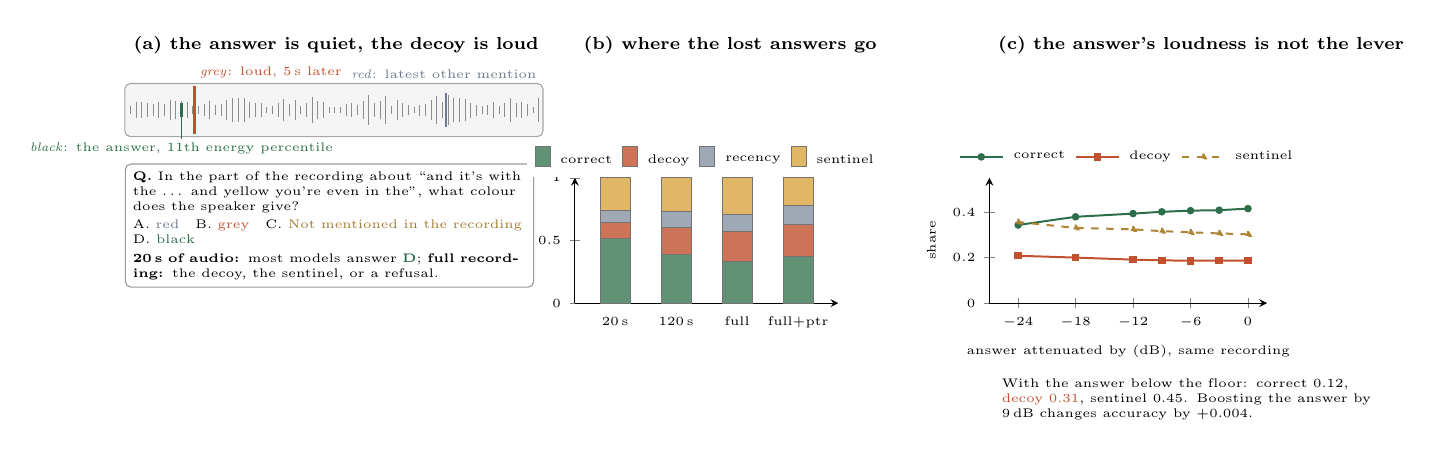
\begin{tikzpicture}[font=\scriptsize,scale=0.90,every node/.style={transform shape}]
\node[font=\scriptsize\bfseries,anchor=south west] at (0,2.05) {(a) the answer is quiet, the decoy is loud};
\draw[rounded corners=2pt,fill=black!4,draw=black!35] (0,1.0) rectangle (5.9,1.75);
\foreach \x in {0.08,0.16,...,5.85}{
  \pgfmathsetmacro{\h}{0.04+0.20*abs(sin(\x r*3.1))*rnd}
  \draw[black!45,line width=0.3pt] (\x,1.375-\h) -- (\x,1.375+\h);}
\draw[csal,line width=1pt] (0.98,1.03) -- (0.98,1.72);
\draw[ccorrect,line width=1pt] (0.80,1.28) -- (0.80,1.47);
\draw[crec,line width=1pt] (4.53,1.14) -- (4.53,1.61);
\node[csal,anchor=south west,inner sep=1pt,font=\tiny] at (1.02,1.78) {\emph{grey}: loud, 5\,s later};
\node[ccorrect,anchor=south,inner sep=1pt,font=\tiny] at (0.80,0.72) {\emph{black}: the answer, 11th energy percentile};
\node[crec,anchor=south east,inner sep=1pt,font=\tiny] at (5.85,1.78) {\emph{red}: latest other mention};
\draw[ccorrect,line width=0.3pt] (0.80,0.96) -- (0.80,1.28);
\node[draw=black!40,rounded corners=2pt,fill=white,inner sep=3pt,anchor=north west,
      text width=5.55cm,font=\tiny] at (0,0.62)
 {\textbf{Q.} In the part of the recording about ``and it's with the \ldots\ and yellow you're
  even in the'', what colour does the speaker give?\\[1.5pt]
  A.~\textcolor{crec}{red} \; B.~\textcolor{csal}{grey} \;
  C.~\textcolor{cabs!75!black}{Not mentioned in the recording} \; D.~\textcolor{ccorrect}{black}\\[1.5pt]
  \textbf{20\,s of audio:} most models answer \textcolor{ccorrect}{\textbf{D}};
  \textbf{full recording:} the decoy, the sentinel, or a refusal.};
\begin{scope}[xshift=6.35cm]
\node[font=\scriptsize\bfseries,anchor=south west] at (0,2.05) {(b) where the lost answers go};
\begin{axis}[
  at={(0,-1.35cm)}, anchor=south west, width=5.3cm,height=3.35cm,
  ybar stacked, bar width=12pt, ymin=0,ymax=1,
  symbolic x coords={L1,L2,L3,L4}, xtick=data,xtick style={draw=none},
  ytick={0,0.5,1.0}, xticklabel style={font=\tiny},yticklabel style={font=\tiny},
  xticklabels={20\,s,120\,s,full,full+ptr}, xlabel style={font=\tiny},
  legend style={font=\tiny,at={(0.5,1.30)},anchor=north,legend columns=4,draw=none,column sep=2pt},
  axis lines=left, enlarge x limits=0.22,
]
\addplot[fill=ccorrect!75,draw=black!55] coordinates {\coordsCorrect};
\addplot[fill=csal!80,draw=black!55]     coordinates {\coordsSalience};
\addplot[fill=crec!65,draw=black!55]     coordinates {\coordsRecency};
\addplot[fill=cabs!80,draw=black!55]     coordinates {\coordsAbsent};
\legend{correct,decoy,recency,sentinel}
\end{axis}
\end{scope}
\begin{scope}[xshift=12.2cm]
\node[font=\scriptsize\bfseries,anchor=south west] at (0,2.05) {(c) the answer's loudness is not the lever};
\begin{axis}[
  at={(0,-1.35cm)}, anchor=south west, width=5.5cm,height=3.35cm,
  ymin=0,ymax=0.55, xmin=-27, xmax=2,
  xtick={0,-6,-12,-18,-24}, ytick={0,0.2,0.4},
  xticklabel style={font=\tiny},yticklabel style={font=\tiny},
  xlabel={answer attenuated by (dB), same recording},xlabel style={font=\tiny},
  ylabel={share},ylabel style={font=\tiny},
  legend style={font=\tiny,at={(0.5,1.30)},anchor=north,legend columns=3,draw=none,column sep=2pt},
  axis lines=left,
]
\addplot[ccorrect,mark=*,mark size=1.1pt,thick] coordinates {\sweepCorrect};
\addplot[csal,mark=square*,mark size=1.1pt,thick] coordinates {\sweepSalience};
\addplot[cabs!80!black,mark=triangle*,mark size=1.2pt,thick,dashed] coordinates {\sweepAbsent};
\legend{correct,decoy,sentinel}
\end{axis}
\node[anchor=north west,font=\tiny,text width=5.3cm,align=left] at (0.05,-2.3)
 {With the answer below the floor: correct \sweeprmCorrect{},
  \textcolor{csal}{decoy \sweeprmSalience{}}, sentinel \sweeprmAbsent{}.
  Boosting the answer by 9\,dB changes accuracy by \boostMean{}.};
\end{scope}
\end{tikzpicture}
\caption{\textbf{The argument in one figure.} (a)~A real item. The answer
\emph{black} sits at the 11th energy percentile of its window; the decoy
\emph{grey} is said five seconds later and louder. Both are inside the
recording, so a model that picks the decoy has not fabricated anything --- it
has mis-selected among heard candidates. (b)~Pooled over the \Nfullcov{}
models that ingest the full window, non-null items: accuracy falls
\roleCorrectLOne{}\,$\rightarrow$\,\roleCorrectLThree{} between a twenty-second clip
and the full recording, and the decoy absorbs most of what is lost; a
timestamp pointer (L4) converts sentinel into decoy rather than into correct.
(c)~Attenuating only the answer, inside a window of its own recording that
holds it and its competitor, from 0 to $-24$\,dB barely moves any share;
pushing it below the room-tone floor does. The loss under context load is
not a loss of audibility.}
\label{fig:teaser}
\end{figure*}

% =====================================================================
\section{Introduction}
\label{sec:intro}

Audio-language models now ingest minutes of speech in a single forward pass,
and a family of benchmarks has grown up to test what they do with it
\cite{airbench,mmau,audiobench,dynamicsuperb}. These benchmarks agree on a
headline: accuracy degrades as recordings lengthen. They disagree on almost
nothing else, because they all report the same quantity --- the fraction of
items answered correctly --- and that quantity is a scalar.

A scalar records that a model failed and discards the evidence about why.
Consider two systems that both answer a third of five-minute retrieval items
correctly. The first spends its errors declaring that the requested fact was
never mentioned; the second spends them confidently reporting a different
value that the same recording contains. These are not variations of one
failure. The first is a search process that terminates without a candidate;
the second is a search process that terminates with the wrong candidate and
reports it as if it were right. They call for different interventions, they
carry different downstream risk --- a meeting summariser that abstains is
annoying, one that substitutes is dangerous --- and a benchmark that reports
the same number for both is blind to the distinction.

The instrument for recovering the distinction is already present in every
multiple-choice benchmark and is thrown away for free. If distractors are
arbitrary, a wrong answer carries no information. If every option carries a
fixed semantic role, the identity of the chosen option \emph{is} a
measurement. This is the whole of our design: each item has four options
whose roles are constant across the benchmark, and we read the error
direction off the choice.

\textbf{The roles.} Each item offers (i)~the \emph{correct} answer, a value
actually spoken in the recording; (ii)~the \emph{decoy}, a different value of
the same kind, from the same recording, spoken more loudly or more often than
the answer; (iii)~the \emph{recency} option, the most recent other mention of
the same kind; and (iv)~a byte-identical \emph{sentinel}, ``Not mentioned in
the recording''. Every one of the first three was said. A model that picks
the decoy has not hallucinated; it has preferred a prominent heard candidate
over a quiet one. A model that picks the sentinel has declined to commit. The
four-way distribution over these roles, which we call the error direction, is
the object this paper measures.

\textbf{What we find.} Fig.~\ref{fig:teaser} previews the result. Presented
with a twenty-second window containing the answer, models choose the decoy
in a minority of cases. Required to retrieve the same answer from its full
recording, they choose it far more often, and the decoy absorbs most of the
accuracy that is lost; every model in the roster --- open, cascaded and
closed --- moves in this direction, and most of the movement happens by two
minutes. A causal arm that attenuates only the answer, inside its own
recording, leaves the outcome unchanged across a 24\,dB range and changes it
only when the answer is pushed below the room-tone floor --- at which point
models split between the loud decoy and the sentinel. Abstention turns out
to be a per-model policy: near-total under silence, model-specific and
insensitive to the audio otherwise; a timestamp pointer converts it into
commitment, which only one closed family converts into correct answers.
Reasoning post-training changes the error direction at fixed size; nominal
parameter count does not.

\noindent\textbf{Contributions.}
\begin{enumerate}\itemsep1.5pt \parskip0pt \leftskip-6pt
\item \textbf{Error-direction measurement.} A role-typed option design that
converts ``which wrong answer'' into a first-class quantity, and derived
metrics --- retrieval cost, substitution share of errors, denial rate,
calibration gap, audio dependence --- that separate substitution from
abstention rather than pooling them (Sec.~\ref{sec:problem}).
\item \textbf{A harvested, stratified benchmark.} Items cut from
real multi-party meetings, never spliced, with the answer in one of five
measured low-prominence configurations; an unanswerable arm as an abstention
control; and an audio-necessity gate that rejects any item a text
system solves from a transcript (Sec.~\ref{sec:bench}).
\item \textbf{A four-arm causal prominence study.} Attenuation and boosting of
the answer, attenuation of its competitor, and a calibrated fine sweep, all
inside a window of the item's own recording that holds both, with the
delivered dose audited, plus a floor level that establishes per-item audio
necessity (Secs.~\ref{ssec:sweep},~\ref{ssec:causal}).
\item \textbf{A ladder that separates hearing from finding.} Within-item
conditions from a twenty-second clip to the full recording and an oracle
pointer, replicated on a separate ten-minute band and on three closed
models (Sec.~\ref{sec:results}).
\item \textbf{Artefact accounting.} Quantification of letter-position
preference, silent encoder truncation, a dead option letter, runaway
reasoning traces and scorer disagreement, each capable of moving role shares
by tens of points if ignored, with the affected rows excluded from every
pooled number rather than averaged in (Sec.~\ref{ssec:artefacts}).
\end{enumerate}

% =====================================================================
\section{Related Work}
\label{sec:related}

\subsection{Long-form audio benchmarks}
General audio-language benchmarks \cite{airbench,mmau,audiobench,dynamicsuperb}
test breadth over short clips. Long-context evaluation in text established the
needle-in-a-haystack paradigm \cite{niah,ruler} and its characteristic
positional failure \cite{lostmiddle}; audio adaptations vary the amount of
audio surrounding a needle whose acoustic properties are held fixed, either
by inserting a clip into a haystack --- where the splice boundary is a cue a
model can exploit --- or by locating a natural span post hoc, where the
needle's prominence is whatever it happened to be. None of them types the
wrong answers. \bench{} inverts the manipulated variable: the amount of
audio is a within-item ladder, the needle's prominence relative to a
competitor is measured and then edited, and the wrong answers are the
measurement.

\subsection{Distractors and multiple-choice robustness}
Multiple-choice evaluation is far less stable than its headline numbers
suggest: models carry letter preferences \cite{mcqselectors}, rephrasing
distractors moves accuracy by many points, and text-only models clear chance
on ostensibly audio benchmarks through language priors alone. That
literature treats the distractor as a confound to be neutralised. We take the
opposite stance: the distractor is the instrument. We fix distractor
\emph{wording} where possible --- the sentinel is a single byte-identical
string on every item, so abstention cannot be identified by lexical drift ---
and control the distractor's \emph{role} instead. Letter is treated as a
nuisance variable to be balanced and reported (Sec.~\ref{ssec:artefacts}).

\subsection{Hallucination and abstention}
Audio hallucination benchmarks measure fabrication: content asserted by a
model that is not present in the signal \cite{audiohallu}. Every non-sentinel
option in \bench{} was actually spoken in the recording, so what we measure is
not fabrication but mis-selection among heard candidates. The two are related
but distinct, and they have different remedies: fabrication is a grounding
problem, mis-selection is a search and weighting problem. The sentinel
connects our design to the abstention literature: it gives the model a
correct action when the evidence is absent, which lets us ask whether the
presence of audio --- any audio --- suppresses justified abstention
(Sec.~\ref{ssec:controls}).

\subsection{Prominence and competing streams}
Work on speech in competing streams varies the signal-to-noise ratio of an
external masker \cite{cherry,bregman}. Our competitor is not an added noise
source but a second utterance from the same conversation, spoken by a
participant, in the same room and channel as the answer. This removes every
acoustic confound that an added stream introduces, and the resulting failure
is one a deployed system will actually make: meetings contain competing
values, and the loud one is not always the operative one. The causal arm
lets us ask the question the masking literature would ask --- does the
answer's level determine whether it is retrieved --- and Sec.~\ref{ssec:causal}
answers it in the negative over a 24\,dB range.

\subsection{Positional effects in long context}
The lost-in-the-middle result \cite{lostmiddle} predicts that long-context
models under-use material in the centre of their input. If that mechanism
transferred to audio, retrieval errors should be attracted to late material,
and specifically to the most recent mention. We include a recency-typed
option precisely so this prediction can be tested rather than assumed;
Sec.~\ref{ssec:overall} reports that recency moves, but by a fraction of
what the decoy moves.

% =====================================================================
\section{Problem Formulation}
\label{sec:problem}

\subsection{Role-typed items}
An item is a tuple $(a, q, \mathcal{O}, \rho)$ where $a$ is a recording, $q$
a question, $\mathcal{O}=\{o_1,\dots,o_4\}$ a set of options, and
$\rho:\mathcal{O}\rightarrow\{\textsc{cor},\textsc{dec},\textsc{rec},
\textsc{abs}\}$ a bijection assigning each option a semantic role. The
assignment of roles to \emph{letters} is drawn from a seeded shuffle per item
and shared across all models and conditions, so that within-item comparisons
are letter-matched.

Let $M$ be a model and $c$ a presentation condition. The measurement is not
the indicator $\mathbb{1}[\hat{o}=o_{\textsc{cor}}]$ but the full
distribution
\[
  \pi_{M,c} \;=\; \big(\pi^{\textsc{cor}},\,\pi^{\textsc{dec}},\,
  \pi^{\textsc{rec}},\,\pi^{\textsc{abs}}\big),
  \qquad \textstyle\sum_r \pi^r = 1 ,
\]
estimated over items. We call $\pi$ the \emph{error direction}; accuracy is
its first coordinate, and the conventional benchmark reports that coordinate
alone.

\subsection{Derived metrics}
Four quantities do the analytical work.

\noindent\textbf{Retrieval cost} $\;\mathcal{R} =
\pi^{\textsc{cor}}_{\textsc{L1}} - \pi^{\textsc{cor}}_{\textsc{L3}}$, the
accuracy lost between a twenty-second window containing the answer and the
full recording. Without the isolated condition, a low long-audio score cannot
be attributed: it confuses failure to hear with failure to find.

\noindent\textbf{Substitution share of errors} $\;\mathcal{S} =
\pi^{\textsc{dec}}/(1-\pi^{\textsc{cor}})$, the fraction of \emph{all} errors
that are substitutions. This is the scale-free form of the central quantity.
The raw decoy share falls mechanically as accuracy rises, so comparing it
across models of different strength measures strength rather than direction;
$\mathcal{S}$ does not have that defect.

\noindent\textbf{Denial rate} $\;\pi^{\textsc{abs}}$ on non-null items, where
choosing the sentinel is by construction an error, paired with sentinel
accuracy on null items, where it is by construction correct. The gap between
the two is a \emph{calibration gap}: a well-calibrated model abstains when
and only when the evidence is absent.

\noindent\textbf{Audio dependence} $\;\mathcal{A} =
\pi^{\textsc{cor}}_{0\text{dB}} - \pi^{\textsc{cor}}_{\text{removed}}$,
measured in the causal arm. $\mathcal{A}>0$ certifies that the item is
answered from the audio rather than from priors in the prompt.

\subsection{What the design holds fixed}
Three confounds are removed by construction rather than by statistical
adjustment. \emph{Splice artefacts}: needles are harvested from the recording
they are asked about, never inserted, so there is no channel, room or
loudness discontinuity at the needle boundary. \emph{Lexical identifiability
of abstention}: the sentinel is one string, repeated verbatim on every item.
\emph{Transcript leakage}: an audio-necessity gate rejects any item that a
text model answers from a transcript. The causal arm goes further and holds
the recording, the speaker and the words constant while changing only the
relative level of the answer, which is as close to an intervention as a
benchmark on real speech can get.

% =====================================================================
\section{The \bench{} Benchmark}
\label{sec:bench}

\subsection{Source}
Audio is drawn from \corpus{} \cite{ami}, the mixed far-field channel, across
its scenario meetings (role-played design meetings) and its non-scenario
meetings (real research meetings). Recordings are cut into consecutive
five-minute windows, each its own haystack; a separate ten-minute band uses
the same harvest at twice the window length. Every result row carries the
pack fingerprint of the item set it was scored against, so a resumed or
extended run cannot silently mix item versions.

\subsection{Needle harvesting}
A needle is a value a speaker actually gave: a colour, a material, a
percentage, a price, a duration, a count. Candidates are located by pattern
over the reference transcript, aligned to audio by word timing, and scored
for the acoustic properties that define the strata below. An item is only
possible where the window contains at least three distinct values of one
\emph{quantity kind} --- colours with colours, percentages with percentages
--- because that is what makes the wrong options competing mentions rather
than fabrications. Harvesting rather than inserting costs yield --- the
conjunction of ``a value was given'' with ``a competing value of the same
kind exists nearby and was said more prominently'' is rare --- but it buys
ecological validity: every configuration in the benchmark is one that
really occurred.

\subsection{Option construction}
The \emph{decoy} is the competing value of the same kind with the highest
repetition count or energy. The \emph{recency} option is the competing value
said last in the window; it may precede or follow the answer, so this role
tests attraction to late mentions rather than to positions after the answer.
The \emph{sentinel} is fixed. Questions quote the words around the needle
with the answer removed, giving every condition an identical lexical anchor
and making the cascaded control in Sec.~\ref{ssec:controls} a fair
comparison.

\subsection{Prominence strata}
\label{ssec:strata}
Each item is assigned the acoustic or lexical reason its answer is hard to
hear, tested in a fixed priority order so that a ubiquitous filler cannot
relabel a masked mention: \textbf{P4} unmarked self-repair (the same speaker
restates a different value within seconds, without ``sorry'' or ``I mean'');
\textbf{P3} backgrounded (the answer is prosodically flat while a competing
value is loud or repeated; a small constructed arm re-mixes real needles to
make this contrast explicit); \textbf{P2} masked (the answer overlaps other
speech); \textbf{P1} quiet (bottom energy percentile of its window);
\textbf{C1} hesitation-adjacent. The strata are the natural yield of the
corpus rather than balanced, and Table~\ref{tab:strata} reports them with
their sizes.

\subsection{Null items}
Null items reuse a sibling item's audio and options but ask for an
attribute of a different kind --- a time or a weight over colour or
percentage options. The values on offer are still spoken in the audio; the
question is what makes none of them an answer, so the sentinel is the only
correct response. They therefore test whether a model will decline a
question whose options do not fit it, with the lure of an audible value on
the table; Sec.~\ref{ssec:controls} shows that no model does so beyond its
own abstention rate.

\subsection{Audio-necessity gate}
Every candidate is rejected if a text model answers it from a transcript.
P1--P3 items are gated on a Whisper \cite{whisper} transcript of the same
audio, because the claim they support is that a cascaded ASR system cannot
solve them; P4 and C1 are gated on the reference transcript, because their
answer genuinely is not in the words --- ASR normalises a repair away and
never records hesitancy. Both leak rates are recorded for every category so
the rate we are not rejecting on is visible.

\begin{table}[t]
\centering\scriptsize
\setlength{\tabcolsep}{3pt}
\caption{Error direction by prominence stratum, pooled over the \Nfullcov{}
full-window models on non-null items. Items: non-null items in the stratum.
20\,s/full: accuracy in the isolated and full conditions;
$\mathcal{R}$: retrieval cost; the last three columns are role shares at
full.}
\label{tab:strata}
\begin{tabular}{@{}lr cc c ccc@{}}
\toprule
Stratum & Items & 20\,s & full & $\mathcal{R}$ & decoy & recency & sentinel \\
\midrule
\catBody
\bottomrule
\end{tabular}
\vspace{-4pt}
\end{table}

% =====================================================================
\section{Experimental Setup}
\label{sec:setup}

\subsection{Models}
We evaluate \Nmodels{} open audio-language models with native audio input
from \Nfamilies{} families, including two matched instruct/thinking pairs
that share a base model and audio encoder, which isolates the effect of
reasoning post-training from the effect of scale (Table~\ref{tab:models}).
Documented audio-input limits range from 30\,s to 30\,min and are enforced
per item. Every pooled number in this paper is computed over the
\Nfullcov{} models whose long-window rows are interpretable: \Ntrunc{}
models cannot ingest beyond 30\,s, and one more behaves as if it did not
(Sec.~\ref{ssec:artefacts}); all \Nexcluded{} are reported in every table
and excluded from every pool. Three closed models are run through their
APIs on the same items and letter maps (Sec.~\ref{ssec:closed}).

\subsection{Conditions}
\textbf{L1} presents a twenty-second window centred on the answer: no search
is required, and the condition functions as a perception ceiling.
\textbf{L2} widens the window to two minutes. \textbf{L3} presents the item's
full window. \textbf{L4} presents L3 plus the timestamp of the answer span,
in a prompt that already quotes the answer's surrounding words; it measures
how much of the loss is localisation rather than reading. Prompt, options
and letter map are identical across the four.

\subsection{Causal prominence arms}
\label{ssec:sweep}
Four edits are applied inside the \emph{contrast window}: the smallest span
of the item's own recording that holds both the answer and its decoy, padded
and capped at 90\,s, so that the competitor is always in earshot and the arm
measures prominence rather than plain audibility. Recording, speaker, words
and every other acoustic property are held fixed; the unedited window is
scored alongside as the 0\,dB control, and every level is read against that
control, not against the ladder. \emph{Attenuation}: only the answer span is
attenuated by 0, $-3$, $-6$, $-9$, $-12$, $-18$ and $-24$\,dB with
raised-cosine ramps, then by a nominal $-60$\,dB. \emph{Boost}: the answer is
raised by $+3$, $+6$ and $+9$\,dB. \emph{Competitor}: the decoy's own
utterance is attenuated by $-6$, $-12$ and $-24$\,dB and then by $-60$\,dB,
on the items whose decoy falls inside the window. \emph{Calibrated}: the
answer is attenuated in 2\,dB steps from 0 to $-12$\,dB. Each row stores the
measured answer-to-decoy contrast after the edit. The delivered dose tracks
the nominal one to $-12$\,dB and saturates near the room-tone floor: the
median achieved contrast change is \achievedTwentyfour{}\,dB at nominal
$-24$ and \achievedSixty{}\,dB at nominal $-60$, so the last level is ``the
answer below the floor'', a binary endpoint rather than a point on the
curve. The arms score every model by letter logits; the two thinking models
answer after a reasoning span and their first-token logits are not their
answer, so their arm rows are excluded and the arms are pooled over the
\Nsweeppool{} logit-scored full-window models.
\subsection{Controls}
\label{ssec:controlsetup}
A \textbf{silence} baseline presents the prompt with twenty seconds of
silence, establishing what the question and options alone support. A
\textbf{cascaded text twin} transcribes the same window with Whisper and
answers with a text LLM on identical items and letter maps
(\Ntwins{} text models), separating what is lost in transcription from what
is lost in selection. The \textbf{null} items supply the abstention control.

\subsection{Scoring}
Models are scored by letter log-likelihood over A--D in a single forward
pass. The two thinking models open a reasoning span before answering and
their letter logits are uninformative, so they are scored by free
generation with strict single-letter parsing, as are the closed models. Where
both scorers are available they agree on \scorerAgree{} of full-window cells
($n=\scorerAgreeN{}$); we report the primary scorer per model rather than
average across them.

\subsection{Compute}
The protocol is \Ncells{} scored cells in total, run in fp16 on single A40
and T4 GPUs, with every row stamped with the pack fingerprint and the code
commit that produced it.

% =====================================================================
\section{Results}
\label{sec:results}

\begin{table*}[t]
\centering\scriptsize
\setlength{\tabcolsep}{3.4pt}
\caption{Per-model results on non-null items. Params: nominal parameter
count from the model card (billions). Limit: documented audio-input ceiling;
\ctr{grey} models hear only the first 30\,s of a long window, so their L2--L4
columns measure truncation, not retrieval, and they are excluded from every
pooled number. Scorer: letter logits or free generation. L1--L4: accuracy.
$\mathcal{R}$: retrieval cost L1$-$L3. Decoy, sentinel: role shares at L3.
$\mathcal{S}$: decoy share of all L3 errors. $\mathcal{A}$: audio dependence
from the causal arm.}
\label{tab:models}
\begin{tabular}{@{}llcclcccc c cc c c@{}}
\toprule
Model & Family & Params & Limit & Scorer & L1 & L2 & L3 & L4 & $\mathcal{R}$ & decoy & sentinel & $\mathcal{S}$ & $\mathcal{A}$ \\
\midrule
\ladderBody
\bottomrule
\end{tabular}
\vspace{-4pt}
\end{table*}

\subsection{The error direction}
\label{ssec:overall}
\finding{Under context load the lost accuracy goes predominantly to the loud
competitor, on every model.}
Pooled over the \Nfullcov{} full-window models and non-null items
(Fig.~\ref{fig:teaser}b), accuracy falls
\roleCorrectLOne{}\,$\rightarrow$\,\roleCorrectLThree{} between L1 and L3, a
retrieval cost of $\mathcal{R}=\retrievalCost{}$ (cluster bootstrap over
windows, 95\% half-width \ciRetrievalCost{}). The decoy share rises
\roleSalienceLOne{}\,$\rightarrow$\,\roleSalienceLThree{}; the substitution share
of errors rises \Siso{}\,$\rightarrow$\,\Sfull{}. At the level of
model$\times$item cells, correct falls on \pairCorrectDown{} and rises on
\pairCorrectUp{} ($p\pairCorrectP{}$), and the decoy rises on
\pairSalienceUp{} and falls on \pairSalienceDown{} ($p\pairSalienceP{}$).
Recency moves less (\roleRecencyLOne{}\,$\rightarrow$\,\roleRecencyLThree{})
and the sentinel least (\roleAbsentLOne{}\,$\rightarrow$\,\roleAbsentLThree{}).
At the model level, L3 accuracy is below L1 accuracy for \signLThreebelowLOne{}
full-window models and \signLThreebelowLOneall{} models overall ($p\signPall{}$,
sign test); the decoy share rises on \signDecoyUp{}; per-model retrieval
cost ranges from \minRetrievalCost{} to \maxRetrievalCost{}
(Table~\ref{tab:models}). The \Ntwins{} text twins and the three closed
models fall and shift the same way (Secs.~\ref{ssec:controls},~\ref{ssec:closed}).

The L1 condition is what makes this interpretable. At twenty seconds the
decoy takes only \roleSalienceLOne{} of choices \emph{even though on most items
it is inside the clip}. The acoustics of answer and decoy are identical in
the two conditions; what differs is how much material lies between them and
around them. The substitution prior is therefore a property of selection
under context load, not of perception --- a conclusion the causal arm makes
directly in Sec.~\ref{ssec:causal}.

\finding{Abstention is a per-model policy, not a response to the audio.}
The sentinel share on non-null items ranges from \absRangeLo{}
(\absLightest{}) to \absRangeHi{} (\absHeaviest{}) across the pooled models
at L1, and for \absPolicyStable{} of them it changes by at most six points
between L1 and L3 (Table~\ref{tab:models}). Under silence the same models
abstain almost perfectly (Sec.~\ref{ssec:controls}). A model's abstention is
thus a threshold it applies to ``I found nothing'', set per model and
largely independent of whether the answer was audible; the marginal error
under load is not a retreat to the sentinel but capture by the decoy.

\subsection{Search load}
\label{ssec:bylen}

\begin{table}[t]
\centering\scriptsize
\setlength{\tabcolsep}{3.5pt}
\caption{Error direction against the amount of audio to be searched. The
first three rows are the same items under widening windows; the last row is
a separate ten-minute band. Items: non-null items scored per model. Mdl:
full-window models pooled.}
\label{tab:len}
\begin{tabular}{@{}llrr cccc@{}}
\toprule
Window & Design & Items & Mdl & correct & decoy & recency & sentinel \\
\midrule
\lenBody
\bottomrule
\end{tabular}
\vspace{-4pt}
\end{table}

\finding{Substitution grows with the amount of audio that must be searched;
most of the growth happens in the first two minutes, and where the answer
sits in the window does not matter.}
Table~\ref{tab:len} and Fig.~\ref{fig:len} trace the same items through
twenty seconds, two minutes and the full five-minute window, then the
separate ten-minute band. The decoy share climbs
\lenSalFirst{}\,$\rightarrow$\,\lenSalLast{} and accuracy falls
\lenCorrFirst{}\,$\rightarrow$\,\lenCorrLast{} across the range. The first
step is the large one: widening twenty seconds to two minutes costs
\poolDropOneTwo{} pooled and the further step to five minutes
\poolDropTwoThree{}, with the first exceeding the second for
\signStepOneTwo{} models. A few additional competing mentions do most of the
damage that the whole window will do. The position of the answer inside the
five-minute window does not predict retrieval: accuracy is
\posAccFirst{}, \posAccMiddle{} and \posAccLast{} for answers in the first,
middle and last third of the window, with no dip in the middle and no
primacy advantage, and recency moves far less than the decoy --- so the
growth is not the positional degradation that long-context text models show
\cite{lostmiddle}.

\begin{table}[t]
\centering\scriptsize
\setlength{\tabcolsep}{2.2pt}
\caption{Five-minute band against the separate ten-minute band, per pooled
model, non-null items: accuracy at L1 and L3, and sentinel and decoy shares
at L3. The two bands hold different items, so rows are anchored on their own
L1.}
\label{tab:band}
\begin{tabular}{@{}l cccc cccc@{}}
\toprule
& \multicolumn{4}{c}{300\,s window} & \multicolumn{4}{c}{600\,s window} \\
\cmidrule(lr){2-5}\cmidrule(lr){6-9}
Model & L1 & L3 & sent. & decoy & L1 & L3 & sent. & decoy \\
\midrule
\bandSwitchBody
\bottomrule
\end{tabular}
\vspace{-4pt}
\end{table}

\finding{Doubling the window again changes the failure mode for some
models: from the wrong value to the sentinel.}
On the ten-minute band (Table~\ref{tab:band}) every pooled model keeps its
twenty-second accuracy and loses more at the full window. For
\NbandSwitch{} models (\bandSwitchNames{}) the extra loss is not a rise in
decoy choices but a jump in the sentinel share to about half of all
answers, and the L4 pointer does not bring them back. Two mechanisms fit:
audio-token positions beyond the trained range degrading the representation,
so the model reports nothing found, or an unchanged encoder with a retrieval
policy that abstains once the search space doubles. Feeding these items as
five-minute windows that still contain the answer and its competitors would
separate them; that experiment is in the pipeline but not in this paper.

\begin{figure}[t]
\centering
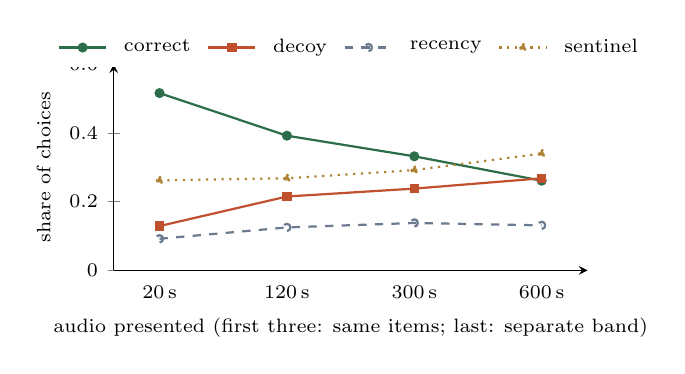
\begin{tikzpicture}
\begin{axis}[
  width=7.6cm,height=4.2cm,
  ymin=0,ymax=0.6, symbolic x coords={20\,s,120\,s,300\,s,600\,s},
  xtick=data,xtick style={draw=none}, ytick={0,0.2,0.4,0.6},
  xticklabel style={font=\scriptsize},yticklabel style={font=\scriptsize},
  ylabel={share of choices},ylabel style={font=\scriptsize},
  xlabel={audio presented (first three: same items; last: separate band)},xlabel style={font=\scriptsize},
  legend style={font=\scriptsize,at={(0.5,1.18)},anchor=north,legend columns=4,draw=none,column sep=4pt},
  axis lines=left, enlarge x limits=0.12,
]
\addplot[ccorrect,mark=*,mark size=1.4pt,thick] coordinates {\lenCorrect};
\addplot[csal,mark=square*,mark size=1.3pt,thick] coordinates {\lenSalience};
\addplot[crec,mark=o,mark size=1.3pt,thick,dashed] coordinates {\lenRecency};
\addplot[cabs!80!black,mark=triangle*,mark size=1.5pt,thick,dotted] coordinates {\lenAbsent};
\legend{correct,decoy,recency,sentinel}
\end{axis}
\end{tikzpicture}
\caption{Role shares against the amount of audio presented, pooled over the
full-window models on non-null items.}
\label{fig:len}
\vspace{-6pt}
\end{figure}

\subsection{The oracle condition}
\label{ssec:oracle}
\finding{A pointer to the answer releases abstention into commitment; only
one closed family converts the commitment into correct answers.}
L4 adds one line to the L3 prompt: the timestamp of the answer span. Pooled
over the open models, denial falls by \oracleDenialDrop{}
(\pairAbsentOracleDown{} cells stop abstaining, \pairAbsentOracleUp{} start,
$p\pairAbsentOracleP{}$; the sentinel share falls for \signOracleAbsDown{}
models) while accuracy rises by only \oracleGain{} (\pairCorrectOracleUp{}
cells become correct, \pairCorrectOracleDown{} become wrong,
$p\pairCorrectOracleP{}$); the decoy share rises from
\roleSalienceLThree{} to \roleSalienceLFour{} (Fig.~\ref{fig:teaser}b). The
largest open-model gain is \openMaxOracleGain{} (\openMaxOracleName{}, the
heaviest abstainer, whose released sentinel mass goes partly to the answer).
The two Gemini models are the exception: their L4 gains are
\closedgeminiflashOracleGain{} and \closedgeminiliteOracleGain{}, bringing
both back to their twenty-second level (Sec.~\ref{ssec:closed}). Even the
\Ntrunc{} models that never receive the audio at the named time cut their
sentinel share at L4, which isolates the prompt-compliance component: ``the
fact is at mm:ss'' suppresses ``not mentioned'' independently of any ability
to seek to mm:ss. The open models that were abstaining did not lack a
location; told the location, most of them pick the loud competitor near
it.

\subsection{The causal prominence arms}
\label{ssec:causal}

\begin{figure}[t]
\centering
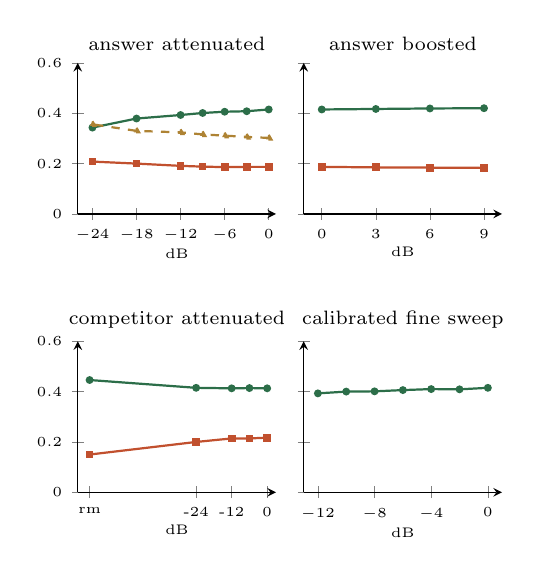
\begin{tikzpicture}
\pgfplotsset{every axis/.style={width=4.1cm,height=3.5cm,ymin=0,ymax=0.6,ytick={0,0.2,0.4,0.6},
  xticklabel style={font=\tiny},yticklabel style={font=\tiny},axis lines=left,
  title style={font=\scriptsize,yshift=-5pt},xlabel style={font=\tiny,yshift=4pt}}}
\begin{axis}[name=att, xmin=-26,xmax=1, xtick={0,-6,-12,-18,-24}, title={answer attenuated}, xlabel={dB}]
\addplot[ccorrect,mark=*,mark size=1pt,thick] coordinates {\sweepCorrect};
\addplot[csal,mark=square*,mark size=1pt,thick] coordinates {\sweepSalience};
\addplot[cabs!80!black,mark=triangle*,mark size=1.1pt,thick,dashed] coordinates {\sweepAbsent};
\end{axis}
\begin{axis}[name=bst, at={(att.east)},anchor=west,xshift=10pt, xmin=-1,xmax=10, xtick={0,3,6,9}, yticklabels={}, title={answer boosted}, xlabel={dB}]
\addplot[ccorrect,mark=*,mark size=1pt,thick] coordinates {\boostCurve};
\addplot[csal,mark=square*,mark size=1pt,thick] coordinates {\boostDecoy};
\end{axis}
\begin{axis}[name=cmp, at={(att.south west)},anchor=north west,yshift=-46pt, xmin=-64,xmax=3, xtick={0,-12,-24,-60}, xticklabels={0,-12,-24,rm}, title={competitor attenuated}, xlabel={dB}]
\addplot[ccorrect,mark=*,mark size=1pt,thick] coordinates {\compCurve};
\addplot[csal,mark=square*,mark size=1pt,thick] coordinates {\compDecoy};
\end{axis}
\begin{axis}[name=cal, at={(cmp.east)},anchor=west,xshift=10pt, xmin=-13,xmax=1, xtick={0,-4,-8,-12}, yticklabels={}, title={calibrated fine sweep}, xlabel={dB}]
\addplot[ccorrect,mark=*,mark size=1pt,thick] coordinates {\calCurve};
\end{axis}
\end{tikzpicture}
\caption{The four causal arms, pooled over the \Nsweeppool{} logit-scored
full-window models on non-null items: correct (green), decoy (orange),
sentinel (yellow, dashed). Every edit is applied inside the contrast window
of the item's own recording with the delivered dose audited. Across a
24\,dB attenuation, a 9\,dB boost and attenuation of the competitor to the
floor, the shares move by a few points; only pushing the answer below the
floor moves them.}
\label{fig:causal}
\vspace{-6pt}
\end{figure}

\begin{table}[t]
\centering\scriptsize
\setlength{\tabcolsep}{4pt}
\caption{Per-model effects in the causal arms, accuracy differences on
non-null items, logit-scored models. $\mathcal{A}$: 0\,dB minus the floor
level. Boost: $+9$\,dB minus 0\,dB. Competitor: competitor at the floor
minus intact. Calibrated: $-12$\,dB minus 0\,dB. \ctr{Grey} rows are the
models excluded from pools; their contrast windows are short enough to be
heard, and their signs agree.}
\label{tab:causal}
\begin{tabular}{@{}lcccc@{}}
\toprule
Model & $\mathcal{A}$ & Boost & Competitor & Calibrated \\
\midrule
\twoByTwoBody
\bottomrule
\end{tabular}
\vspace{-4pt}
\end{table}

\finding{Every model depends on the audio, and none depends on the answer's
level: the dose--response is flat, then a cliff at the floor; boosting buys
nothing; silencing the competitor buys almost nothing.}
Pushing the answer below the floor costs accuracy on \signAudioDep{} pooled
models (and \signAudioDepAll{} logit-scored models including the excluded
ones), $\mathcal{A}$ from \audioDepMin{} to \audioDepMax{} (mean
\audioDepMean{}), which certifies that the items are answered from the
audio. But the path to that endpoint is flat: pooled accuracy is
\sweepCorrz{} at 0\,dB, \sweepCorrmTwelve{} at $-12$\,dB and
\sweepCorrmTwentyfour{} at $-24$\,dB (an achieved change of
\achievedTwentyfour{}\,dB), then \sweepCorrmSixty{} at the floor
(Fig.~\ref{fig:causal}, top left): a drop of \cliffDrop{} over the last few
achieved decibels after almost none over the first twenty. There is no
graded audibility regime; the answer is either still decodable or gone. The
calibrated arm, whose delivered dose is exact, gives a mean change of
\calMean{} at $-12$\,dB (\signCal{} models negative). Boosting the answer by
9\,dB changes accuracy by \boostMean{} on average (range \boostMin{} to
\boostMax{}). Attenuating the decoy's own utterance to the floor raises
accuracy by \compMean{} (\signComp{} models positive) and lowers the decoy
share only from \compDecoyZero{} to \compDecoyRemoved{}: the decoy is still
chosen at nearly that rate when its loudest utterance is inaudible, so the
choice is carried by its other mentions and by the prior, not by the loud
token, and the freed mass goes to the sentinel and to recency rather than
to the answer. The competitor is not masking the answer.

Taken with Sec.~\ref{ssec:overall}, this locates the failure. The same
answer, at the same level, is retrieved from twenty seconds and lost from
five minutes; changing its level by 24\,dB changes nothing; only making it
disappear does. Audio encoders normalise level, so a $-24$\,dB word is still
a word. The models are not failing to \emph{hear} a quiet answer. They are
failing to \emph{select} it once enough competing material surrounds it,
and the selection is insensitive to the acoustic property the strata were
built around.

\finding{With the answer below the floor, models do not guess it; they split
between the loud decoy and the sentinel, in model-specific proportions.}
At the floor the correct option is chosen on \sweeprmCorrect{} of cells,
below chance --- models do not guess a value they did not hear --- while the
decoy takes \sweeprmSalience{} (up \sweepDecoyRise{} from 0\,dB, rising for
\signSweepDecoyUp{} models) and the sentinel \sweeprmAbsent{} (up
\sweepDenialRise{}, rising for \signSweepDenialUp{}). Which of the two
absorbs the lost mass is a model trait --- the heavy abstainers go to the
sentinel, the committed answerers to the decoy --- and the decoy share at
the floor is the cleanest single measurement of the ``loudest mention
wins'' prior, because it is taken with the answer out of contention.

\subsection{Prominence strata}
\label{ssec:strata_results}
Table~\ref{tab:strata} resolves the error direction by the acoustic reason
the answer is hard. Retrieval cost is largest for stratum \catRmaxName{}
($\mathcal{R}=\catRmaxVal{}$) and smallest for \catRminName{}
(\catRminVal{}); the decoy share at full is highest for \catDecMaxName{}
(\catDecMaxVal{}) and lowest for \catDecMinName{} (\catDecMinVal{}). Every
stratum shows the same direction --- accuracy down, decoy up, from L1 to L3
--- and the strata converge at the full window: the labels mostly describe
how hard the answer is at twenty seconds, and the context cost then closes
the gap. The lexical stratum C1 is neither easier nor harder than the
acoustic ones at L1. Read against Sec.~\ref{ssec:causal}, a quiet answer is
lost under load, but making it louder does not bring it back; the strata
sort items by how much the \emph{context} costs, not by how much the level
costs.

\subsection{Controls}
\label{ssec:controls}

\begin{table}[t]
\centering\scriptsize
\setlength{\tabcolsep}{4pt}
\caption{Silence control. Cells: valid question-only cells. Acc: accuracy on
non-null items with silence in place of audio. Sentinel: sentinel share on
non-null items (an error) and on null items (correct).}
\label{tab:silence}
\setlength{\tabcolsep}{3pt}
\begin{tabular}{@{}lrccc@{}}
\toprule
Model & Cells & Acc & Sent.\ (non-null) & Sent.\ (null) \\
\midrule
\qoBody
\bottomrule
\end{tabular}
\vspace{-4pt}
\end{table}

\finding{Under silence the models abstain almost perfectly; under audio,
null accuracy is just the model's abstention rate.}
With twenty seconds of silence in place of the recording, pooled accuracy on
non-null items is \qoPoolAcc{} and the sentinel takes \qoPoolSentinel{} of
choices; on null items it takes \qoNullSentinel{} (Table~\ref{tab:silence}).
The question and options do not leak the answer, the models can tell silence
from speech, and the sentinel is their response to it. With the full
recording present, the sentinel takes \roleAbsentLThree{} of non-null
choices and \nullSentinelLThree{} of null choices: a calibration gap of
\calibGapLThree{}. On null items the audible lure --- the value of the
sibling item, which the question does not ask for --- is chosen on
\nullLureLOne{} of cells at L1 and \nullLureLThree{} at L3. Across every
model in the study, null accuracy and the non-null sentinel rate are almost
the same quantity (Spearman $\rho=\nullSpearman{}$ over \nullSpearmanN{}
models): the best null score among the open models belongs to the heaviest
abstainer (\nullBestOpenName{}, \nullBestOpen{}), and the strongest content
models choose the lure on most null items. No model detects the absence of
an answer as such; a grounded model answers with the value it heard, and
what looks like abstention calibration is the per-model policy of
Sec.~\ref{ssec:overall}.

\begin{table}[t]
\centering\scriptsize
\setlength{\tabcolsep}{4pt}
\caption{Cascaded text twins on identical items, windows and letter maps:
Whisper transcript in place of the audio. Accuracy at L1 and L3, retrieval
cost, decoy and sentinel shares at L3, non-null items.}
\label{tab:twins}
\begin{tabular}{@{}lccc cc@{}}
\toprule
Cascade & L1 & L3 & $\mathcal{R}$ & decoy & sentinel \\
\midrule
\twinBody
\bottomrule
\end{tabular}
\vspace{-4pt}
\end{table}

\finding{A cascade loses the answer in the same direction, and an
end-to-end audio model beats its own text twin pairwise.}
Given the same windows as transcripts, all \Ntwins{} text models fall from
L1 to L3 (\signTwinDrop{}; pooled
\twinCorrOne{}\,$\rightarrow$\,\twinCorrThree{}) and all shift toward the
decoy (\signTwinDecoyUp{}; pooled decoy share \twinDecoyThree{} at L3,
Table~\ref{tab:twins}): the substitution prior is not confined to the audio
pathway, it is a property of selecting among competing values in a long
context, and it appears in text models given a gapped quote and a
five-minute transcript. The audio-necessity gate is what keeps the twins
near chance on the acoustic strata (Appendix~\ref{app:twincat}). Pairing an
open audio model with the cascade built on its own text-model family, the
audio model is right where the text twin is wrong on \twinPairAudioRight{}
items and the reverse on \twinPairTextRight{} ($p\twinPairP{}$), and the two
pipelines fail on largely different items: the audio pathway carries
information the transcript has lost, and loses it again under load.

\subsection{Closed models}
\label{ssec:closed}

\begin{table}[t]
\centering\scriptsize
\setlength{\tabcolsep}{2.2pt}
\caption{Closed models through their APIs, scored by generation, non-null
items. Items: items with a valid L1 cell. Refusals: full-window cells on
which the model declined to answer at all (not counted in any share).
GPT-audio-mini was run at L1 and L3 only.}
\label{tab:closed}
\begin{tabular}{@{}lr cccc c cc r@{}}
\toprule
Model & Items & L1 & L2 & L3 & L4 & $\mathcal{R}$ & decoy & sent. & Ref. \\
\midrule
\closedBody
\bottomrule
\end{tabular}
\vspace{-4pt}
\end{table}

\finding{Two closed families reproduce the direction; the strongest model
loses less, loses it the same way, and is the only one that can use a
timestamp.}
Gemini 3.5 Flash is the strongest model in the study at every condition
(\closedgeminiflashCorrOne{}\,$\rightarrow$\,\closedgeminiflashCorrThree{})
and still loses accuracy on \closedgeminiflashPairDown{} items against
\closedgeminiflashPairUp{} ($p\closedgeminiflashPairP{}$), with the same
shift toward the decoy; its lighter sibling and GPT-audio-mini show the same
paired asymmetry (Table~\ref{tab:closed}). What separates the Gemini models
is L4: gains of \closedgeminiflashOracleGain{} and
\closedgeminiliteOracleGain{}, uniform over where the answer sits, against
at most \openMaxOracleGain{} for any open model. Two mechanisms fit ---
genuine timestamp-addressable audio tokens, or the same prompt-compliance
effect landing on a model whose content answers are mostly right --- and an
L4 with a deliberately wrong timestamp would separate them. GPT-audio-mini
adds a failure mode absent from every open model: on
\closedgptaudiominiRefusals{} full-window non-null items it declines to
answer, in most cases stating that it cannot identify a speaker from a voice
sample, and on none of the twenty-second clips; the refusals concentrate in
the overlapped (\refusPTwo{}) and self-repair (\refusPFour{}) strata. The
trigger is the length of the audio, not the question, which is identical in
both conditions.

\subsection{Scale and post-training}
\label{ssec:byscale}

\begin{figure}[t]
\centering
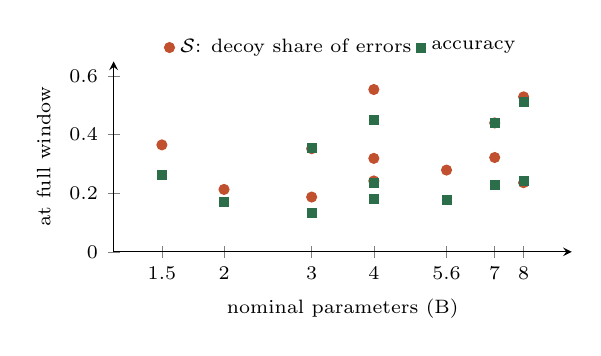
\begin{tikzpicture}
\begin{axis}[
  width=7.4cm,height=4.0cm, xmode=log, log basis x=2,
  xmin=1.2,xmax=10, ymin=0,ymax=0.65,
  xtick={1.5,2,3,4,5.6,7,8}, xticklabels={1.5,2,3,4,5.6,7,8},
  xticklabel style={font=\scriptsize},yticklabel style={font=\scriptsize},
  xlabel={nominal parameters (B)},xlabel style={font=\scriptsize},
  ylabel={at full window},ylabel style={font=\scriptsize},
  legend style={font=\scriptsize,at={(0.5,1.18)},anchor=north,legend columns=2,draw=none},
  axis lines=left,
]
\addplot[only marks,mark=*,mark size=1.8pt,csal] coordinates {\scaleCoords};
\addplot[only marks,mark=square*,mark size=1.6pt,ccorrect] coordinates {\scaleAccCoords};
\legend{$\mathcal{S}$: decoy share of errors, accuracy}
\end{axis}
\end{tikzpicture}
\caption{Neither the substitution share of errors nor accuracy tracks
nominal parameter count across the \NscaleModels{} models with a stated
size ($r=\rSalErrSize{}$, $p=\pSalErrSize{}$ and $r=\rAccSize{}$,
$p=\pAccSize{}$ against $\log$ parameters).}
\label{fig:scale}
\vspace{-6pt}
\end{figure}

\finding{Parameter count predicts neither accuracy nor error direction
across the roster; within a family, size helps a little at the full window
and reasoning post-training helps a lot at every window.}
Across the \NscaleModels{} models with a stated size, $\mathcal{S}$ spans
\salErrLo{} to \salErrHi{} with no relation to $\log$ parameters
($r=\rSalErrSize{}$, $p=\pSalErrSize{}$), and accuracy is no better
predicted ($r=\rAccSize{}$, $p=\pAccSize{}$; Fig.~\ref{fig:scale}). Within
a family the larger variant is no better at twenty seconds and somewhat
better at the full window (Table~\ref{tab:pairs}). The matched
instruct/thinking pairs are decisive. At 4B, the thinking variant abstains on
\mossFourbThinkDen{} of full-window items against \mossFourbInstDen{} for
its instruct sibling, with accuracy \mossFourbThinkCorr{} against
\mossFourbInstCorr{}; at 8B, \mossEightbThinkDen{} against
\mossEightbInstDen{} and \mossEightbThinkCorr{} against
\mossEightbInstCorr{}. Reasoning post-training converts denial into
commitment, and the commitment is right often enough to raise accuracy ---
but the substitution share of errors \emph{rises} with it
(\mossFourbInstS{}\,$\rightarrow$\,\mossFourbThinkS{} and
\mossEightbInstS{}\,$\rightarrow$\,\mossEightbThinkS{}): what the thinking
model no longer denies, it more often substitutes.

\begin{table}[t]
\centering\scriptsize
\setlength{\tabcolsep}{4pt}
\caption{Size within a family: smaller / larger variant, non-null items.
Accuracy at L1 and L3 and the substitution share of errors at L3.}
\label{tab:pairs}
\begin{tabular}{@{}lccc@{}}
\toprule
Pair & L1 & L3 & $\mathcal{S}$ \\
\midrule
\sizePairBody
\bottomrule
\end{tabular}
\vspace{-4pt}
\end{table}

\subsection{Artefacts}
\label{ssec:artefacts}
Five artefacts would each move role shares by tens of points if ignored.
None is averaged in; each is measured and its rows are excluded from the
pools.

\textbf{Letter position.} Pooled at L3, the most and least chosen letters take
\letterMax{} and \letterMin{} of choices; the sentinel is chosen at
\sentinelLetterMax{} when it sits at its favourite letter and
\sentinelLetterMin{} at its least (Fig.~\ref{fig:letters}). The per-item
seeded shuffle spreads each role evenly over letters, so the artefact cancels
in every pooled share, but any subgroup analysis must check that it still
does.

\textbf{Encoder truncation.} The \Ntrunc{} models with a 30\,s ceiling
hear only the first 30\,s of a long window. Their apparent retrieval cost is
\truncCorrOne{}\,$\rightarrow$\,\truncCorrThree{}, the largest in the study,
but on the items whose answer falls inside the first 30\,s they score
\truncInsideCorr{} at L3 against \truncOutsideCorr{} elsewhere, with denial
\truncOutsideDen{}. This is a measurement of the encoder limit, not of
long-audio understanding, and pooling these models with the rest would
quietly attribute the limit to retrieval. They are reported in
Table~\ref{tab:models} and excluded from every pooled number.

\textbf{A dead option.} Aero-1-Audio chooses one of the four letters on
well under one percent of its cells, so a quarter of every item set is
unanswerable for it whatever it hears; its per-cell latency is also the same
at twenty seconds and at five minutes, whereas every other full-window model
takes several times longer on the long window. Its long-window rows are
reported in Table~\ref{tab:models} and treated as those of a truncated
model.

\textbf{Runaway reasoning.} The thinking models occasionally fail to emit
an answer, producing repeated sentences until the generation budget ends;
these cells are counted as unparsed, not wrong, and their number grows with
the window (\unparsedThinkFourb{} and \unparsedThinkEightb{} cells at
L1--L4 for the 4B and 8B variants).

\textbf{Scorer.} For the logit-scored models the free generation agrees with
the letter argmax on \scorerAgree{} of full-window cells. Thinking models and
API models can only be scored by generation, and the thinking models' first-
token logits are not their answer, which is why their rows are excluded from
the causal arms. The ladder and the causal arms also draw different letter
maps for the same item, so item-level agreement between the two is not
expected and no claim in this paper compares them cell by cell; every level
in an arm is read against that arm's own 0\,dB control.

\begin{figure}[t]
\centering
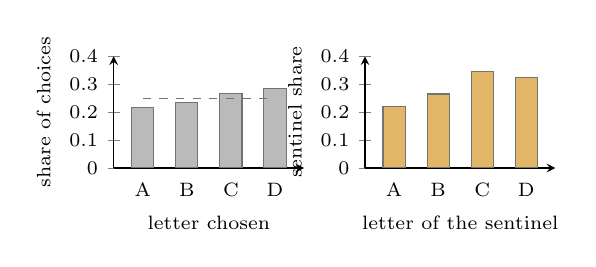
\begin{tikzpicture}
\begin{axis}[
  name=lt, width=4.0cm,height=3.0cm,
  ybar,bar width=8pt, symbolic x coords={A,B,C,D},
  xtick=data,xtick style={draw=none}, ymin=0,ymax=0.4,
  xticklabel style={font=\scriptsize},yticklabel style={font=\scriptsize},
  ylabel={share of choices},ylabel style={font=\scriptsize},
  xlabel={letter chosen},xlabel style={font=\scriptsize},
  axis lines=left,enlarge x limits=0.22,
]
\addplot[fill=cgrey!60,draw=black!55] coordinates {\letterBars};
\draw[black!55,dashed] (axis cs:A,0.25) -- (axis cs:D,0.25);
\end{axis}
\begin{axis}[
  at={(lt.east)},anchor=west,xshift=22pt,
  width=4.0cm,height=3.0cm,
  ybar,bar width=8pt, symbolic x coords={A,B,C,D},
  xtick=data,xtick style={draw=none}, ymin=0,ymax=0.4,
  xticklabel style={font=\scriptsize},yticklabel style={font=\scriptsize},
  ylabel={sentinel share},ylabel style={font=\scriptsize},
  xlabel={letter of the sentinel},xlabel style={font=\scriptsize},
  axis lines=left,enlarge x limits=0.22,
]
\addplot[fill=cabs!80,draw=black!55] coordinates {\sentinelByLetter};
\end{axis}
\end{tikzpicture}
\caption{Letter artefacts at L3, pooled over full-window models. Left: overall
letter preference against the 0.25 line. Right: how often the sentinel is
chosen as a function of the letter it was assigned.}
\label{fig:letters}
\vspace{-6pt}
\end{figure}

% =====================================================================
\section{Discussion}
\label{sec:discussion}

\subsection{What the results imply about mechanism}
Four observations converge on a single account. The decoy is rarely chosen
at twenty seconds even when it is present in the clip; its share grows with
the amount of audio around the answer; a timestamp pointer converts denial
into commitment without proportionally restoring accuracy; and the answer's
own level, over a 24\,dB range, does not matter. Together these say that
when a model must locate the queried value in a long representation,
candidate selection is weighted by something like the number and prominence
of \emph{mentions}, not by the audibility of the one that is correct, and
that the weighting is not corrected by the lexical anchor the question
supplies. The competitor arm sharpens this: silencing the decoy's loud
utterance leaves the decoy chosen almost as often, so the prior that favours
it is carried by its repetition and by the model's expectation, not by the
loud token. A natural next test is mechanistic: cross-attention mass at the
answering step should concentrate on decoy mentions at long durations and on
the answer span at short ones, on the same items. The causal arm supplies
the contrastive pairs that make that test cheap.

\subsection{Implications for evaluation practice}
Four practices follow directly. First, report an isolated condition
alongside any long-audio score; without it a low number cannot be attributed
to search rather than hearing. Second, report at least two numbers:
retrieval cost and substitution share of errors. The second is scale-free,
which the raw decoy share is not, and the pair is small enough to fit in a
leaderboard column. Third, report coverage. Three of the models in this
study cannot ingest a five-minute recording and a fourth behaves as if it
cannot; scoring them alongside models that can, and pooling the result,
produces a benchmark that quietly measures encoder limits and calls it
long-audio understanding. Fourth, rank models, not items: pairwise agreement
on which items are solved is low at the full window (mean Cohen's
$\kappa=\kappaMean{}$, range \kappaMin{}--\kappaMax{}, across the pooled
models; \itemsNoneLThree{} of \itemsCommon{} common items are solved by
none and \itemsAllLThree{} by all), so item difficulty is model-specific
and a fixed ``hard subset'' would encode one model's failures.

\subsection{Implications for model development}
The scale result has direct practical content: within this roster the
substitution prior is not removed by parameter count, and the post-training
recipe that most improves accuracy --- reasoning --- does so by converting
abstentions into commitments, a fraction of which are substitutions. An
intervention aimed at the prior itself would need contrastive material, and
the causal arm supplies it in the form the problem actually takes: the same
item with the answer present and with it removed, and with the competitor
present and with it removed. Any such intervention must be evaluated on both
axes; a model tuned to abstain less will look better on accuracy and worse
on substitution, and a scalar will not show the trade.

\subsection{Why the two failures should never be pooled}
A summarisation system that abstains produces an incomplete summary; a user
notices the gap. A system that substitutes produces a fluent summary
containing a value the speaker said loudly and then corrected; the user
notices nothing. The self-repair stratum makes this concrete: it is where the
decoy share is highest, and it is exactly the case where the loud value is
the one the speaker withdrew. Two systems with identical accuracy can carry
very different downstream risk, and only the error direction distinguishes
them.

% =====================================================================
\section{Limitations}
\label{sec:limits}

\textbf{Meetings, in English.} Every item is cut from \corpus{}
(Appendix~\ref{app:corpus}), in English. The material spans role-played and
real meetings, and the error direction is the same in both
(Appendix~\ref{app:scenario}), but the harvest selects for conversations
that discuss several values of one kind, which is a real and common
configuration and not a random sample of speech. The pipeline is
corpus-agnostic --- a loader that yields time-aligned, speaker-labelled
segments is the only corpus-specific component --- and extension to
\plannedcorpus{} is the first item of future work.

\textbf{The model axis is small.} Every cross-model claim rests on
\Nmodels{} open systems and three closed ones. The scale analysis in
particular cannot be strengthened by collecting more items, and the largest
nominal size is 8B. Claims of the form ``post-training predicts behaviour
better than scale'' should be read as descriptive of this roster.

\textbf{Two scorers.} Thinking and API models are scored by generation and
others by letter log-likelihood. The scorers agree on most cells, so any
comparison that crosses the scorer boundary carries the residual
disagreement.

\textbf{Strata are defined by measured proxies.} ``Quiet'', ``masked'' and
``backgrounded'' are operationalised by energy percentile, overlap and
prosodic flatness. These are correlates of perceptual prominence, not
prominence itself, and the causal arm shows that at least one of them ---
level --- is not what the models are sensitive to. The hesitation stratum
asks a value question with a hesitancy-marked target, a weaker instrument
than a question about delivery.

\textbf{Closed models are partial.} The API runs cover the ladder for one
Gemini model fully and one partially, and only two conditions for
GPT-audio-mini; no causal arm was run through an API.

\textbf{The causal arms are not the ladder.} The arms edit a contrast
window of at most 90\,s, not the five-minute window, because the competitor
has to be in earshot for the edit to mean anything. Their 0\,dB rows are
therefore a separate condition, scored with their own letter map, and every
arm result is a within-arm contrast. The claim they license is about the
answer's level, and it transfers to the ladder only through the argument of
Sec.~\ref{ssec:causal}, not by identity of the audio.

\textbf{Null items are attribute traps.} Their audible lure is by design;
a null item that removed every candidate value from the audio would test a
different ability --- detecting that a fact was never stated --- and this
benchmark does not contain such items.

% =====================================================================
\section{Conclusion and Future Work}
\label{sec:conclusion}

Fixing the semantic role of every option converts an accuracy figure into an
error direction, and the direction turns out to be systematic rather than
noise. A substitution prior toward the prominent competitor is small when the
answer is presented in isolation, grows with the amount of audio to be
searched, is untouched by a 24\,dB change in the answer's own level, survives
deletion of the answer in preference to a correct abstention, is amplified
rather than removed by reasoning post-training, is invariant to parameter
count in this roster, and appears in two closed families. A denial response
is well calibrated under silence and suppressed by audio whether or not the
audio answers the question. These are different problems with different
fixes, and a benchmark that reports one number cannot tell them apart.

\textbf{Future work}, in the order we would pursue it. \emph{(i)~Coverage:}
the same harvest over \plannedcorpus{}, which adds real civic and research
meetings and tests whether the direction survives a change of corpus.
\emph{(ii)~Mechanism:} attention-level verification of the selection account,
using the contrastive pairs the causal arm already produces.
\emph{(iii)~Mitigation:} training on those pairs for prominence invariance,
evaluated on both axes rather than on accuracy. \emph{(iv)~Reporting:} a
two-number score --- retrieval cost and substitution share of errors --- that
a leaderboard can carry without collapsing back to a scalar.

% =====================================================================
\begin{thebibliography}{99}\footnotesize\itemsep0pt
\bibitem{airbench} Q.~Yang et al., ``AIR-Bench: benchmarking large audio-language models via generative comprehension,'' in \emph{ACL}, 2024.
\bibitem{mmau} S.~Sakshi et al., ``MMAU: a massive multi-task audio understanding and reasoning benchmark,'' in \emph{ICLR}, 2025.
\bibitem{audiobench} B.~Wang et al., ``AudioBench: a universal benchmark for audio large language models,'' in \emph{NAACL}, 2025.
\bibitem{dynamicsuperb} C.-y. Huang et al., ``Dynamic-SUPERB: towards a dynamic, collaborative, and comprehensive instruction-tuning benchmark for speech,'' in \emph{ICASSP}, 2024.
\bibitem{niah} G.~Kamradt, ``Needle in a haystack: pressure testing LLMs,'' 2023. \url{https://github.com/gkamradt/LLMTest_NeedleInAHaystack}
\bibitem{ruler} C.-P. Hsieh et al., ``RULER: what's the real context size of your long-context language models?'' in \emph{COLM}, 2024.
\bibitem{lostmiddle} N.~F. Liu et al., ``Lost in the middle: how language models use long contexts,'' \emph{TACL}, 2024.
\bibitem{mcqselectors} C.~Zheng et al., ``Large language models are not robust multiple choice selectors,'' in \emph{ICLR}, 2024.
\bibitem{audiohallu} C.-Y. Kuan et al., ``Understanding sounds, missing the questions: the challenge of object hallucination in large audio-language models,'' in \emph{Interspeech}, 2024.
\bibitem{cherry} E.~C. Cherry, ``Some experiments on the recognition of speech, with one and with two ears,'' \emph{J. Acoust. Soc. Am.}, 1953.
\bibitem{bregman} A.~S. Bregman, \emph{Auditory Scene Analysis}. MIT Press, 1990.
\bibitem{whisper} A.~Radford et al., ``Robust speech recognition via large-scale weak supervision,'' in \emph{ICML}, 2023.
\bibitem{ami} J.~Carletta et al., ``The AMI meeting corpus: a pre-announcement,'' in \emph{MLMI}, 2006.
\end{thebibliography}

\appendix
% =====================================================================
\section{Stability of the aggregates under subsampling}
\label{app:stability}
To check that the pooled findings are not carried by particular items, we
drew 200 random subsets of half the item set, keeping whole windows together
so that the cluster structure is preserved, and recomputed the aggregates on
each. The pooled retrieval cost is \subDeltaFull{} on the full set and lies
between \subDeltaLo{} and \subDeltaHi{} in 95\% of half-size subsets; the
decoy share at L3 is \subSalFull{} against \subSalLo{}--\subSalHi{}; and the
number of full-window models whose accuracy falls from L1 to L3 never drops
below \subSignMin{} of \Nfullcov{}. The headline direction is fixed by the
effect size, not by the item count; what additional items buy is resolution
on the small effects of Sec.~\ref{ssec:causal} and on per-stratum cells.

\section{Packs and clusters}
\label{app:packs}
The item set was built in two disjoint packs with different stratum mixes.
At the full window no pooled model differs between packs (\packSig{} at
$p<0.05$, two-proportion test on L3 accuracy), so they are pooled with pack
kept as a column. Items that share a window share audio, but sharing does
not make them co-fail: the intraclass correlation of L3 correctness within
window ranges from \iccLo{} to \iccHi{} across the pooled models, so the
cluster-robust tests reported above are close to their i.i.d. counterparts.

\section{Scenario and non-scenario meetings}
\label{app:scenario}
On the role-played scenario meetings, pooled accuracy falls
\ScenCorrOne{}\,$\rightarrow$\,\ScenCorrThree{} with a decoy share of
\ScenDec{} and sentinel \ScenDen{} at L3; on the real non-scenario meetings,
\NonscenCorrOne{}\,$\rightarrow$\,\NonscenCorrThree{}, decoy \NonscenDec{},
sentinel \NonscenDen{}. The non-scenario items are fewer and their
strata mix differs, so the two are reported rather than compared; the
direction is the same in both.

\section{By corpus}
\label{app:corpus}
\begin{table}[h]
\centering\scriptsize
\setlength{\tabcolsep}{3pt}
\caption{Error direction by source corpus, pooled over the full-window
models on non-null items; same columns as Table~\ref{tab:strata}.}
\begin{tabular}{@{}lr cc c ccc@{}}
\toprule
Corpus & Items & 20\,s & full & $\mathcal{R}$ & decoy & recency & sentinel \\
\midrule
\corpusBody
\bottomrule
\end{tabular}
\end{table}

\section{Text twins by stratum}
\label{app:twincat}
\begin{table}[h]
\centering\scriptsize
\setlength{\tabcolsep}{5pt}
\caption{Accuracy and sentinel share at L3 by stratum, audio models against
cascaded text twins, non-null items.}
\begin{tabular}{@{}lcc cc@{}}
\toprule
& \multicolumn{2}{c}{accuracy} & \multicolumn{2}{c}{sentinel} \\
\cmidrule(lr){2-3}\cmidrule(lr){4-5}
Stratum & audio & text & audio & text \\
\midrule
\twinCatBody
\bottomrule
\end{tabular}
\end{table}
The audio-necessity gate keeps the text twins near chance on the acoustic
strata by construction; where they clear it, the transcript happened to
retain a recoverable trace of the value.

\end{document}
